% \section{Appendix / supplemental material}

% Optionally include supplemental material (complete proofs, additional experiments and plots) in appendix.
% All such materials \textbf{SHOULD be included in the main submission.}


\newpage
\appendix
\section*{Appendix}

\renewcommand{\thesection}{\Alph{section}} % Optional: Keep if you liked this numbering

% --- titletoc Appendix ToC Start ---
\startcontents[appendix] % Start collecting info for a ToC named 'appendix'
\section*{Appendix Contents} % Add an unnumbered title for this ToC
\printcontents[appendix] % Print the ToC named 'appendix'
               {}{1} % Format: {} = no prefix, {} = default formatting, 1 = start at level 1 (section)
               {\setcounter{tocdepth}{2}} % Set depth to 1 (only sections). Use 2 for subsections etc.
\clearpage
% --- titletoc Appendix ToC End ---


\section{Implementation Details}


\subsection{RLVR Algorithms}
\label{appendix:rlvr_algos}
To reduce memory and computational overhead, several critic-free variants have been proposed.
GRPO~\cite{shao2024deepseekmath} estimates the advantage with a normalized reward within a group of responses to the same question:
$
A_i = [r_i - \operatorname{mean}(\textbf{r})]/{\operatorname{std}(\textbf{r})}$,
where $\textbf{r} = \{r_1, \ldots, r_G\}$
denotes the set of rewards for a group of $G$ sampled responses.
RLOO~\cite{ahmadian2024rloo} instead adopts a leave-one-out baseline within each batch $\mathcal{B}$. Its advantage is defined as
$A_i = r_i - \tfrac{1}{|\mathcal{B}| - 1} \sum_{j \neq i} r_j$.

\subsection{Low-Variance \textit{pass@$k$} Estimation}
\label{appendix:passk_est}
Directly computing pass@$k$ using only $k$ sampled outputs per problem can lead to high variance.  
To mitigate this, we follow the unbiased estimation method proposed by Chen \etal~\cite{chen2021evaluating}.  
Specifically, for each problem $x_i$ from the evaluation dataset $\mathcal{D}$, we generate $n$ samples ($n \geq k$) and count the number of correct samples as $c_i$.  
The unbiased estimator of pass@$k$ over the dataset is given by:
\begin{equation}
\setlength\abovedisplayskip{2pt}
\setlength\belowdisplayskip{2pt}
\text{pass@}k := \mathbb{E}_{x_i \sim \mathcal{D}} \left[ 1 - \frac{\binom{n - c_i}{k}}{\binom{n}{k}} \right]
\end{equation}
With this formulation, we can easily estimate pass@$k$ with low variance across all $k \leq n$.

In our experiments, we set $n$ to the largest (\ie, rightmost) $k$ value in the pass@$k$ curves, typically 128, 256, or 1024. For example, in~\cref{fig:math}, we use $n = 128$ for MATH500, Minerva, and GSM8K, and $n = 1024$ for AMC23 and AIME24. For the Olympiad benchmark, we set $n = 128$ for the Qwen models and $n = 1024$ for LLaMA-3.1-8B, due to its relatively lower base model capacity.







% \vspace{-3mm}
\section{More Related Works}
% \vspace{-2mm}
\label{appendix:more-related}

\noindent\textbf{Reinforcement Learning for LLM Reasoning.}
Since the emergence of LLMs, the post-training phase has proven crucial to enhance problem solving and reasoning abilities~\cite{ouyang2022training}. This stage typically falls into three main categories: supervised fine-tuning using human-curated or distilled data~\cite{wang2023far}, self-improvement iteration~\cite{zelikman2022star, gulcehre2023reinforced}, and reinforcement learning~\cite{ouyang2022training}.
Previously, a reward model or preferences between responses were employed for reward modeling~\cite{ouyang2022training, rafailov2023dpo}.
Recently, Reinforcement Learning with Verifiable Rewards (RLVR) has gained significant traction as a method to improve the reasoning capabilities of LLMs in domains such as mathematics and programming~\cite{lambert2024tulu3,shao2024deepseekmath}. 
An encouraging landmark work is OpenAI's o1 model~\cite{jaech2024openaio1}, which was among the first large-scale applications of RL for reasoning, achieving state-of-the-art results at the time of its release.
Following this, Deepseek-R1~\cite{guo2025deepseek-r1} became the first open-weight model to match or surpass the performance of o1. 
A significant innovation introduced with R1 is the ``zero'' setting, where reinforcement learning is applied directly to the base LLM, bypassing any intermediate supervised tuning.
This approach inspired a wave of open-source efforts to replicate or extend R1's methodology and improve RL algorithms~\cite{zeng2025simplerl, liu2025oat, yu2025dapo, code-r1, zhao2025absolute, wang2025beyond}.
In parallel, reinforcement learning has also gained attention in the multimodal domain, driving advancements in multimodal reasoning~\cite{chen2025r1v, shen2025vlmr1, zheng2025easyr1}.

% analysis: no aha-moment, xxx
\textbf{Analysis of RLVR}. Although there are many excellent open-source works and algorithmic designs in the field of RLVR, there remains a lack of deep understanding regarding the root effects of RLVR on LLM reasoning abilities and its limitations when starting from the base model. 
Several studies~\cite{liu2025there, zhao2025echo, shah2025rethinking} highlight that the reflective behaviors observed in R1-like models actually emerge from the base models, rather than being introduced by RLVR training.
Dang \etal~\cite{dang2025assessing} observed a phenomenon similar to our findings: Pass@k deteriorates rapidly and fails to recover with reinforcement learning, but this was seen only in a limited experimental setup with Qwen-2.5-0.5B on GSM8K. More importantly, they did not explore the relationship between the base model and the RL model. In contrast, our paper conducts systematic and rigorous experiments to show that not only reflective behaviors but all reasoning paths are already embedded in the base model. We further demonstrate that RLVR does not elicit any new reasoning abilities beyond the base model.




% \section{Discussion}
% \label{sec:discuss}
% In~\cref{sec:exp} and~\cref{sec:deep_analysis}, we identified key limitations of RLVR in enhancing LLM reasoning capabilities. In this section, we explore possible underlying factors that may explain why RLVR remains bounded by the reasoning capacity of the base model.

% \textbf{Discussion 1: Key Differences Between Traditional RL and RLVR for LLMs are Vast Action Space and Pretrained Priors.}
% Traditional RL such as AlphaGo Zero and the DQN series~\cite{silver2017alphagozero,mnih2015dqn,yue2023value} can continuously improve the performance of a policy in environments like Go and Atari games \textit{without an explicit upper bound}. There are two key differences between traditional RL and RLVR for LLMs.
% First, the action space in language models is exponentially larger than that of Go or Atari games~\cite{rl4nlp}. 
% RL algorithms were not originally designed to handle such a vast action space, which makes it nearly impossible to explore the reward signal effectively if training starts from scratch. 
% Therefore, the second distinction is that RLVR for LLMs starts with a pretrained base model with useful prior, whereas traditional RL in Atari and GO games often begins from scratch. 
% This pretrained prior guides the LLM in generating reasonable responses, making the exploration process significantly easier, and the policy can receive positive reward feedback.

% \textbf{Discussion 2: Priors as a Double-Edged Sword in This Vast Action Space.}
% Since the sampling of responses is guided by the pretrained prior, the policy may struggle to explore new reasoning patterns beyond what the prior already provides. 
% Specifically, in such a complex and highly combinatorial space, most responses generated during training are constrained by the base model's prior. Any sample deviating from the prior is highly likely to produce invalid or non-sensical outputs, leading to negative reward.
% As discussed in~\cref{sec:prelim}, policy gradient algorithms aim to maximize the log-likelihood of responses within the prior that receive positive rewards, while minimizing the likelihood of responses outside the prior that receive negative rewards. As a result, the trained policy tends to produce responses already present in the prior, constraining its reasoning ability within the boundaries of the base model.
% From this perspective, training RL models from a distilled model may temporarily provide a beneficial solution, as distillation helps inject a better prior. 

% \textbf{Possible Future Work.}
% Developing more efficient exploration strategies may be essential for navigating the vast action space, facilitating the discovery of out-of-prior reasoning patterns and the development of more capable reasoning models. 
% Furthermore, current RLVR frameworks are limited to single-turn interactions with the verifier, lacking the ability to iteratively revise or improve based on environmental feedback. A multi-turn RL agent paradigm---with richer, ongoing interaction with a grounded environment---could enable models to generate novel experiences and learn from them. This agent paradigm has been described as the beginning of an ``era of experience''~\cite{silver2025welcome}.


% \clearpage
\section{Detailed Experimental Results}

% The unfolded y-axis version of~\cref{fig:algo_and_step} is provided in~\cref{fig:algo_and_step_unfold}, and the detailed values of pass@1 and pass@256 are given in~\cref{tab:algos} and~\cref{tab:grpo_training_steps}. Indices of solvable problems in AIME24 and LiveCodeBench are provided in~\cref{tab:sovable_aime24} and~\cref{tab:solvable_livecodebench}.
% Pass@$k$ curves in the filtered AIME24 are shown in~\cref{fig:filtered_aime24}.
% The effects of different temperature settings are shown in~\cref{fig:different_T}.


\subsection{More Results on Mathematics and Coding}
\label{appendix:math}

\begin{figure}[H]
  \centering
      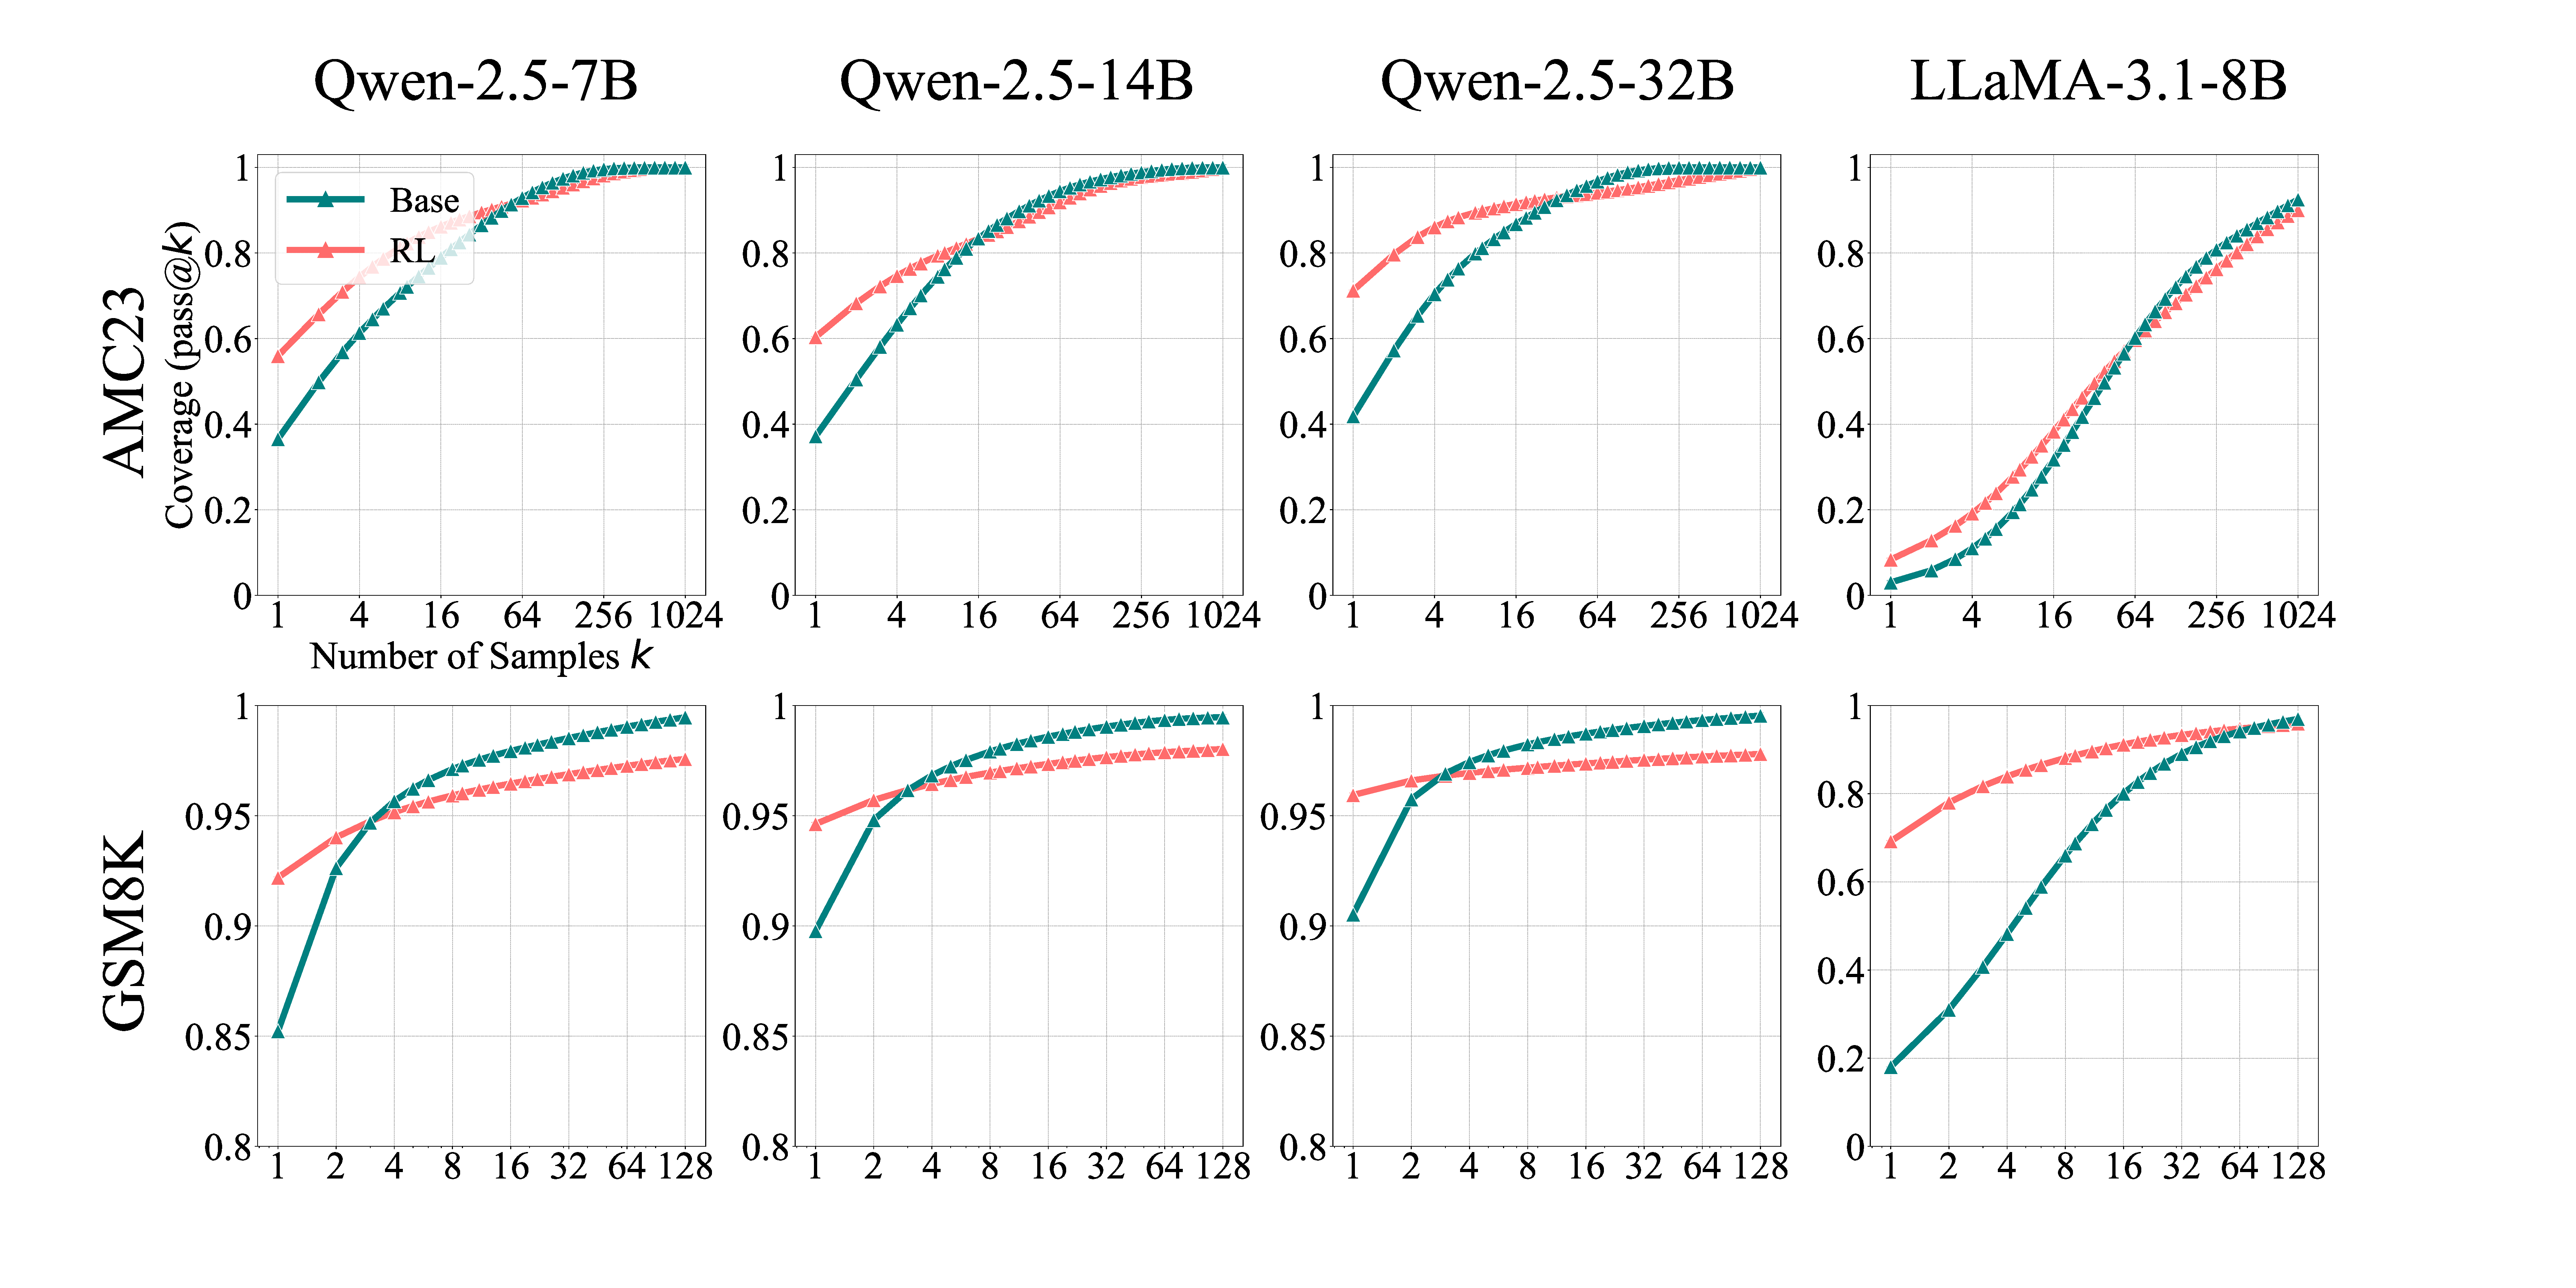
\includegraphics[width=0.95\textwidth]{tex/images/simpleRL_coverage_appendix.pdf}
% \captionsetup{font={footnotesize}}
\caption{
More results of SimpleRLZoo on GSM8K and AMC23.
}
\label{fig:mat_appendix}
\vspace{-3mm}
\end{figure}


\begin{figure}[H]
  \centering
  \begin{subfigure}[b]{0.27\textwidth}
    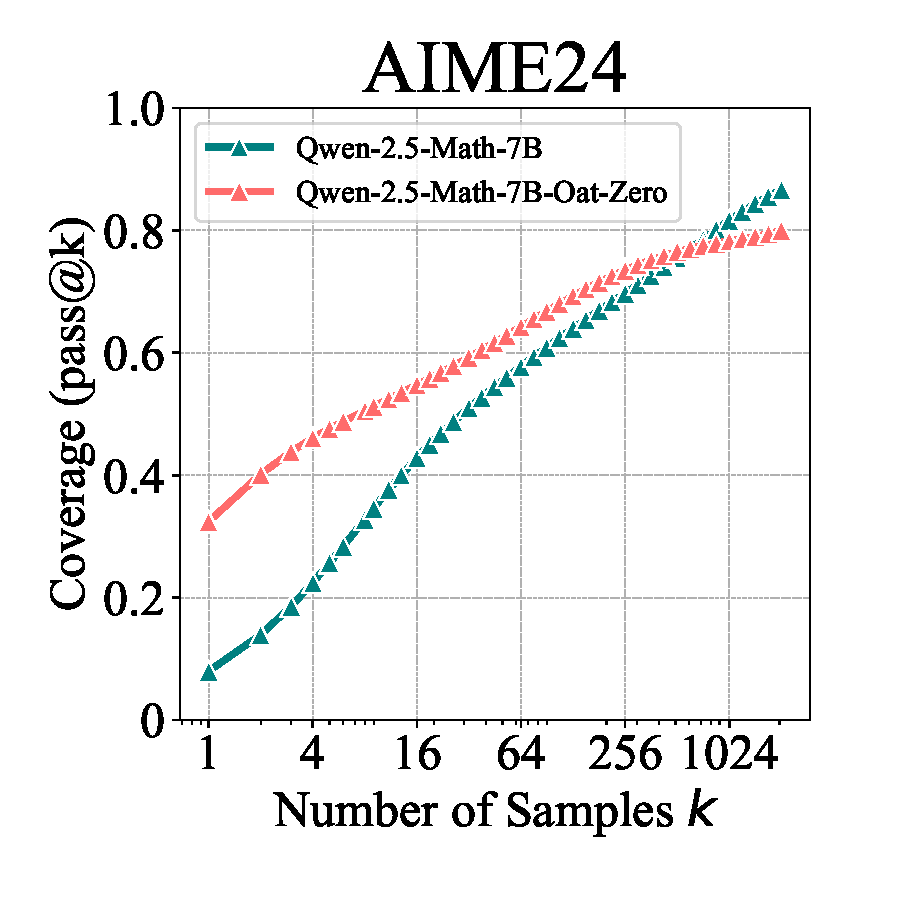
\includegraphics[width=\textwidth]{tex/images/aime24_coverage_oat.pdf}
  \end{subfigure}
  \begin{subfigure}[b]{0.27\textwidth}
    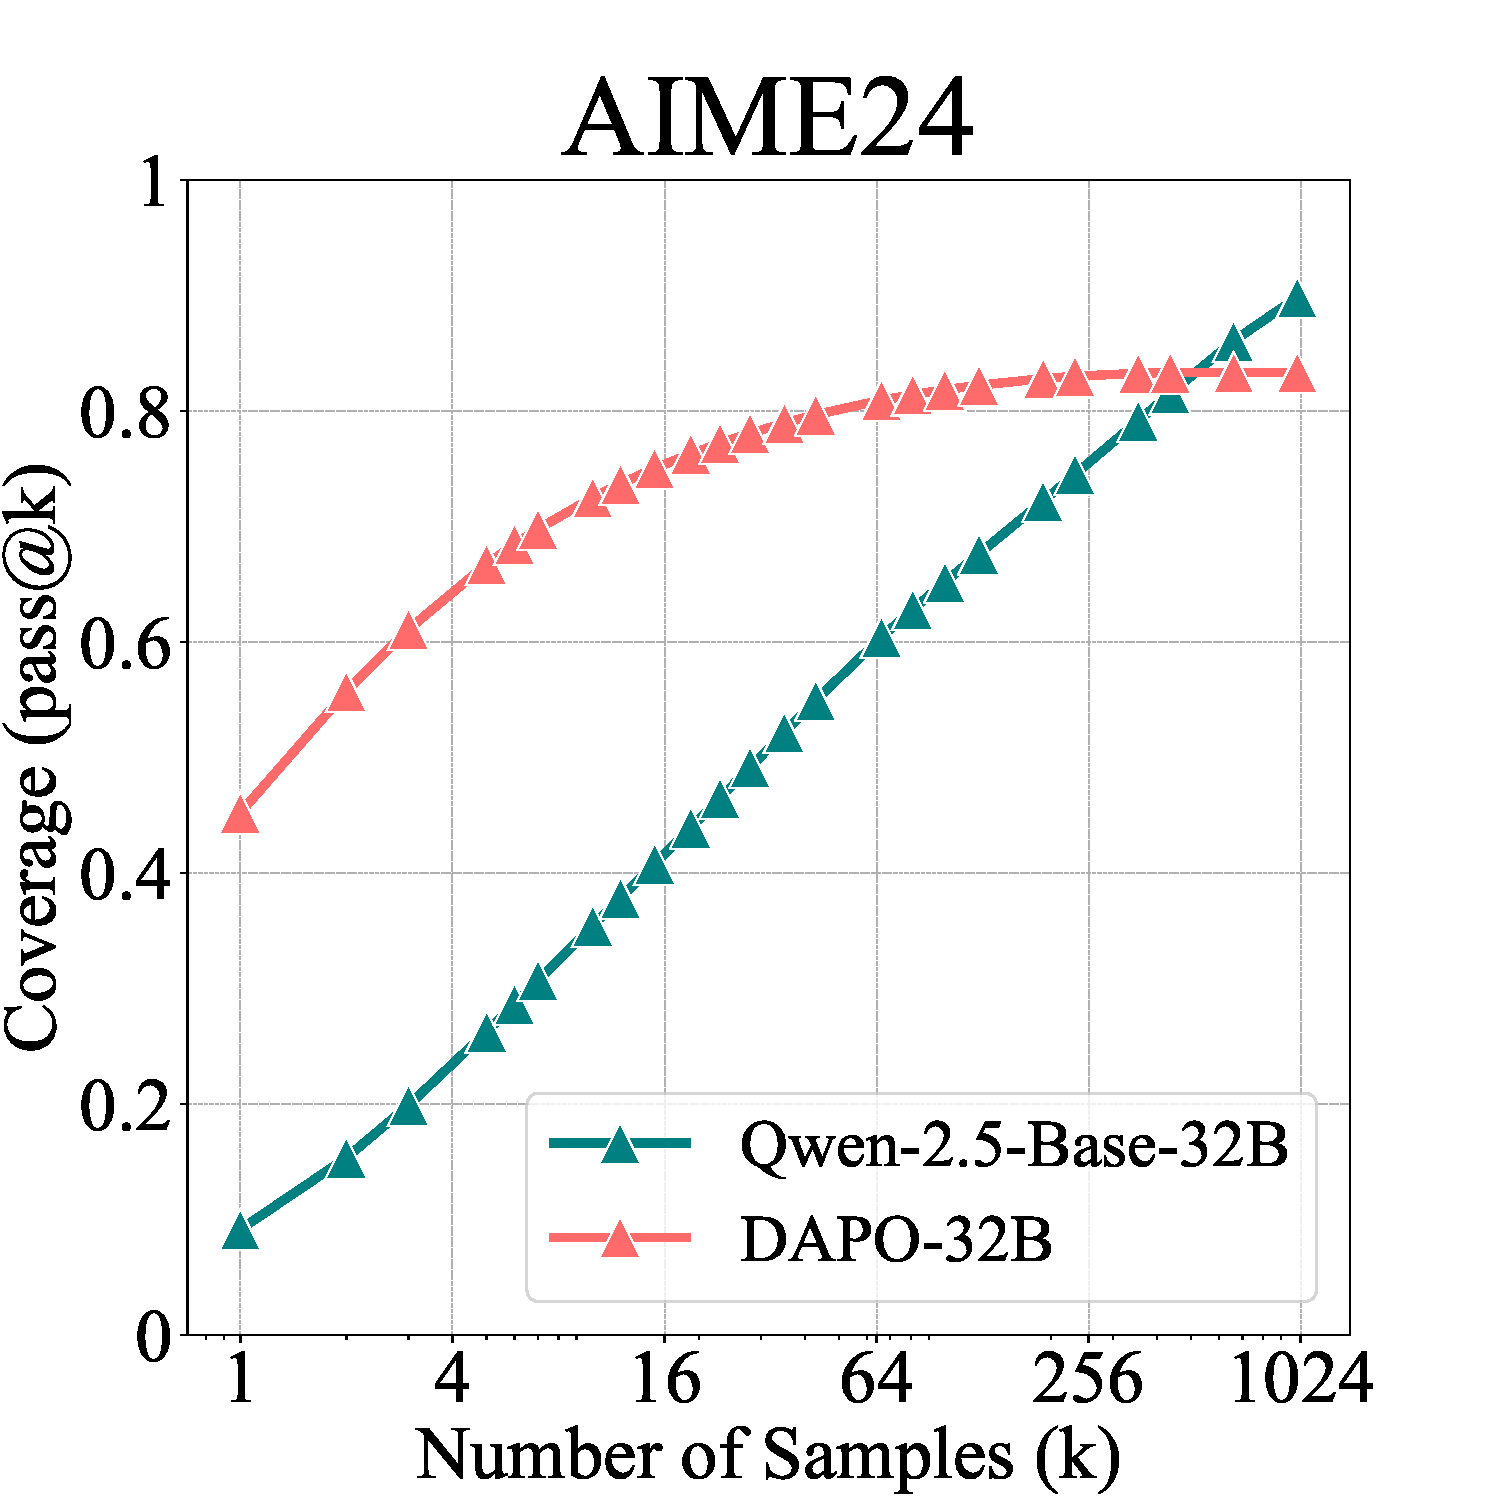
\includegraphics[width=\textwidth]{tex/images/simpleRL_coverage_DAPO.pdf}
  \end{subfigure}
% \captionsetup{font={footnotesize}}
\caption{
Oat-Zero-7B and DAPO-32B are evaluated on AIME24 and compared against their respective base models.
}
\label{fig:oat_aime}
\vspace{-3mm}
\end{figure}


\begin{figure}[H]
  \centering
  \begin{subfigure}[b]{0.3\textwidth}
    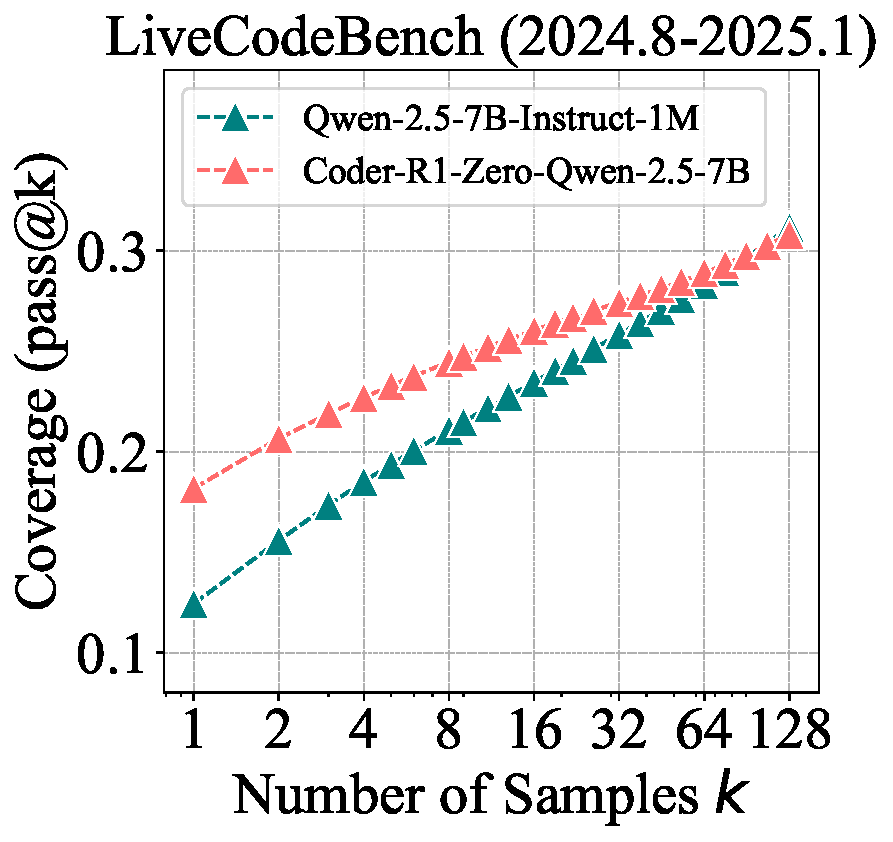
\includegraphics[width=\textwidth]{tex/images/livecodebench_qwen_7b_instruct_coverage_2024-08-01_2025-02-01.pdf}
  \end{subfigure}
  \begin{subfigure}[b]{0.3\textwidth}
    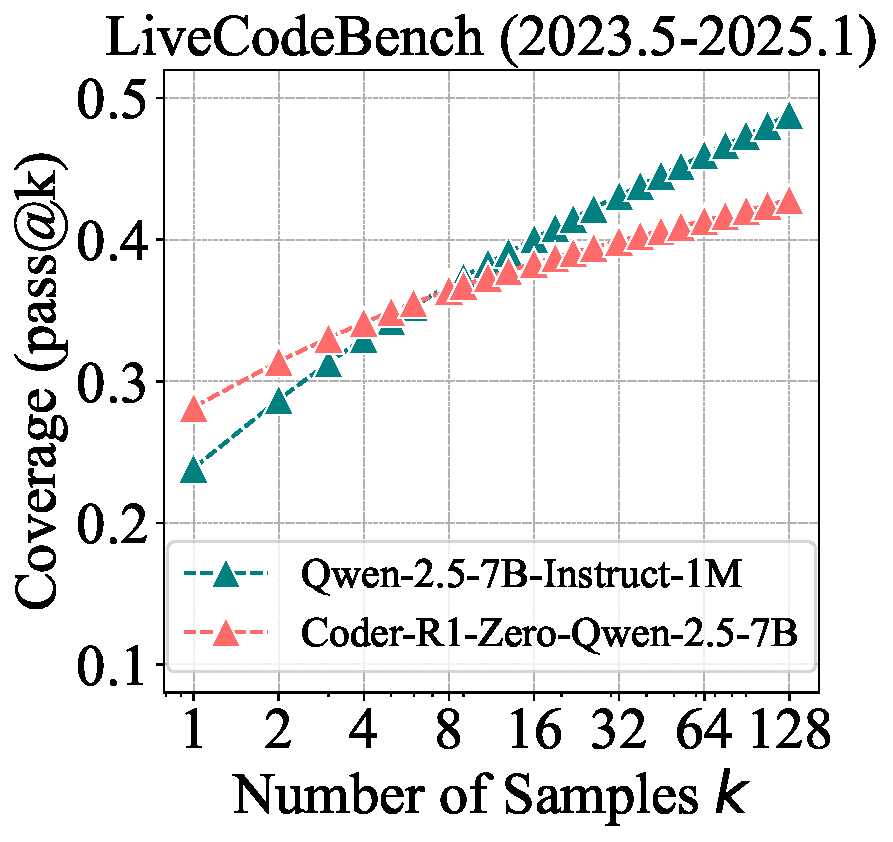
\includegraphics[width=\textwidth]{tex/images/livecodebench_qwen_7b_instruct_coverage.pdf}
  \end{subfigure}
% \captionsetup{font={footnotesize}}
\caption{
Coder-R1 on LiveCodeBench.
}
\label{fig:coder_r1}
\vspace{-3mm}
\end{figure}

\subsection{Validity of Chain-of-Thought on AIME24}
\label{appendix:cot_aime24}

We manually check the CoTs for the most challenging AIME24 benchmark. 
To begin, we introduce a filtering mechanism designed to eliminate easily guessable problems. Specifically, we prompt Qwen2.5-7B-Base to answer questions directly, without using chain-of-thought reasoning, and sample answers multiple times. If a problem can be answered correctly with a low but non-zero probability (e.g., <5\%), we consider it to be guessable and remove it. Problems that can be directly answered correctly with a high probability are retained, as they are likely easier and solvable using valid CoTs.


\begin{figure}[!h]
  \centering
  \begin{subfigure}[b]{0.32\textwidth}
    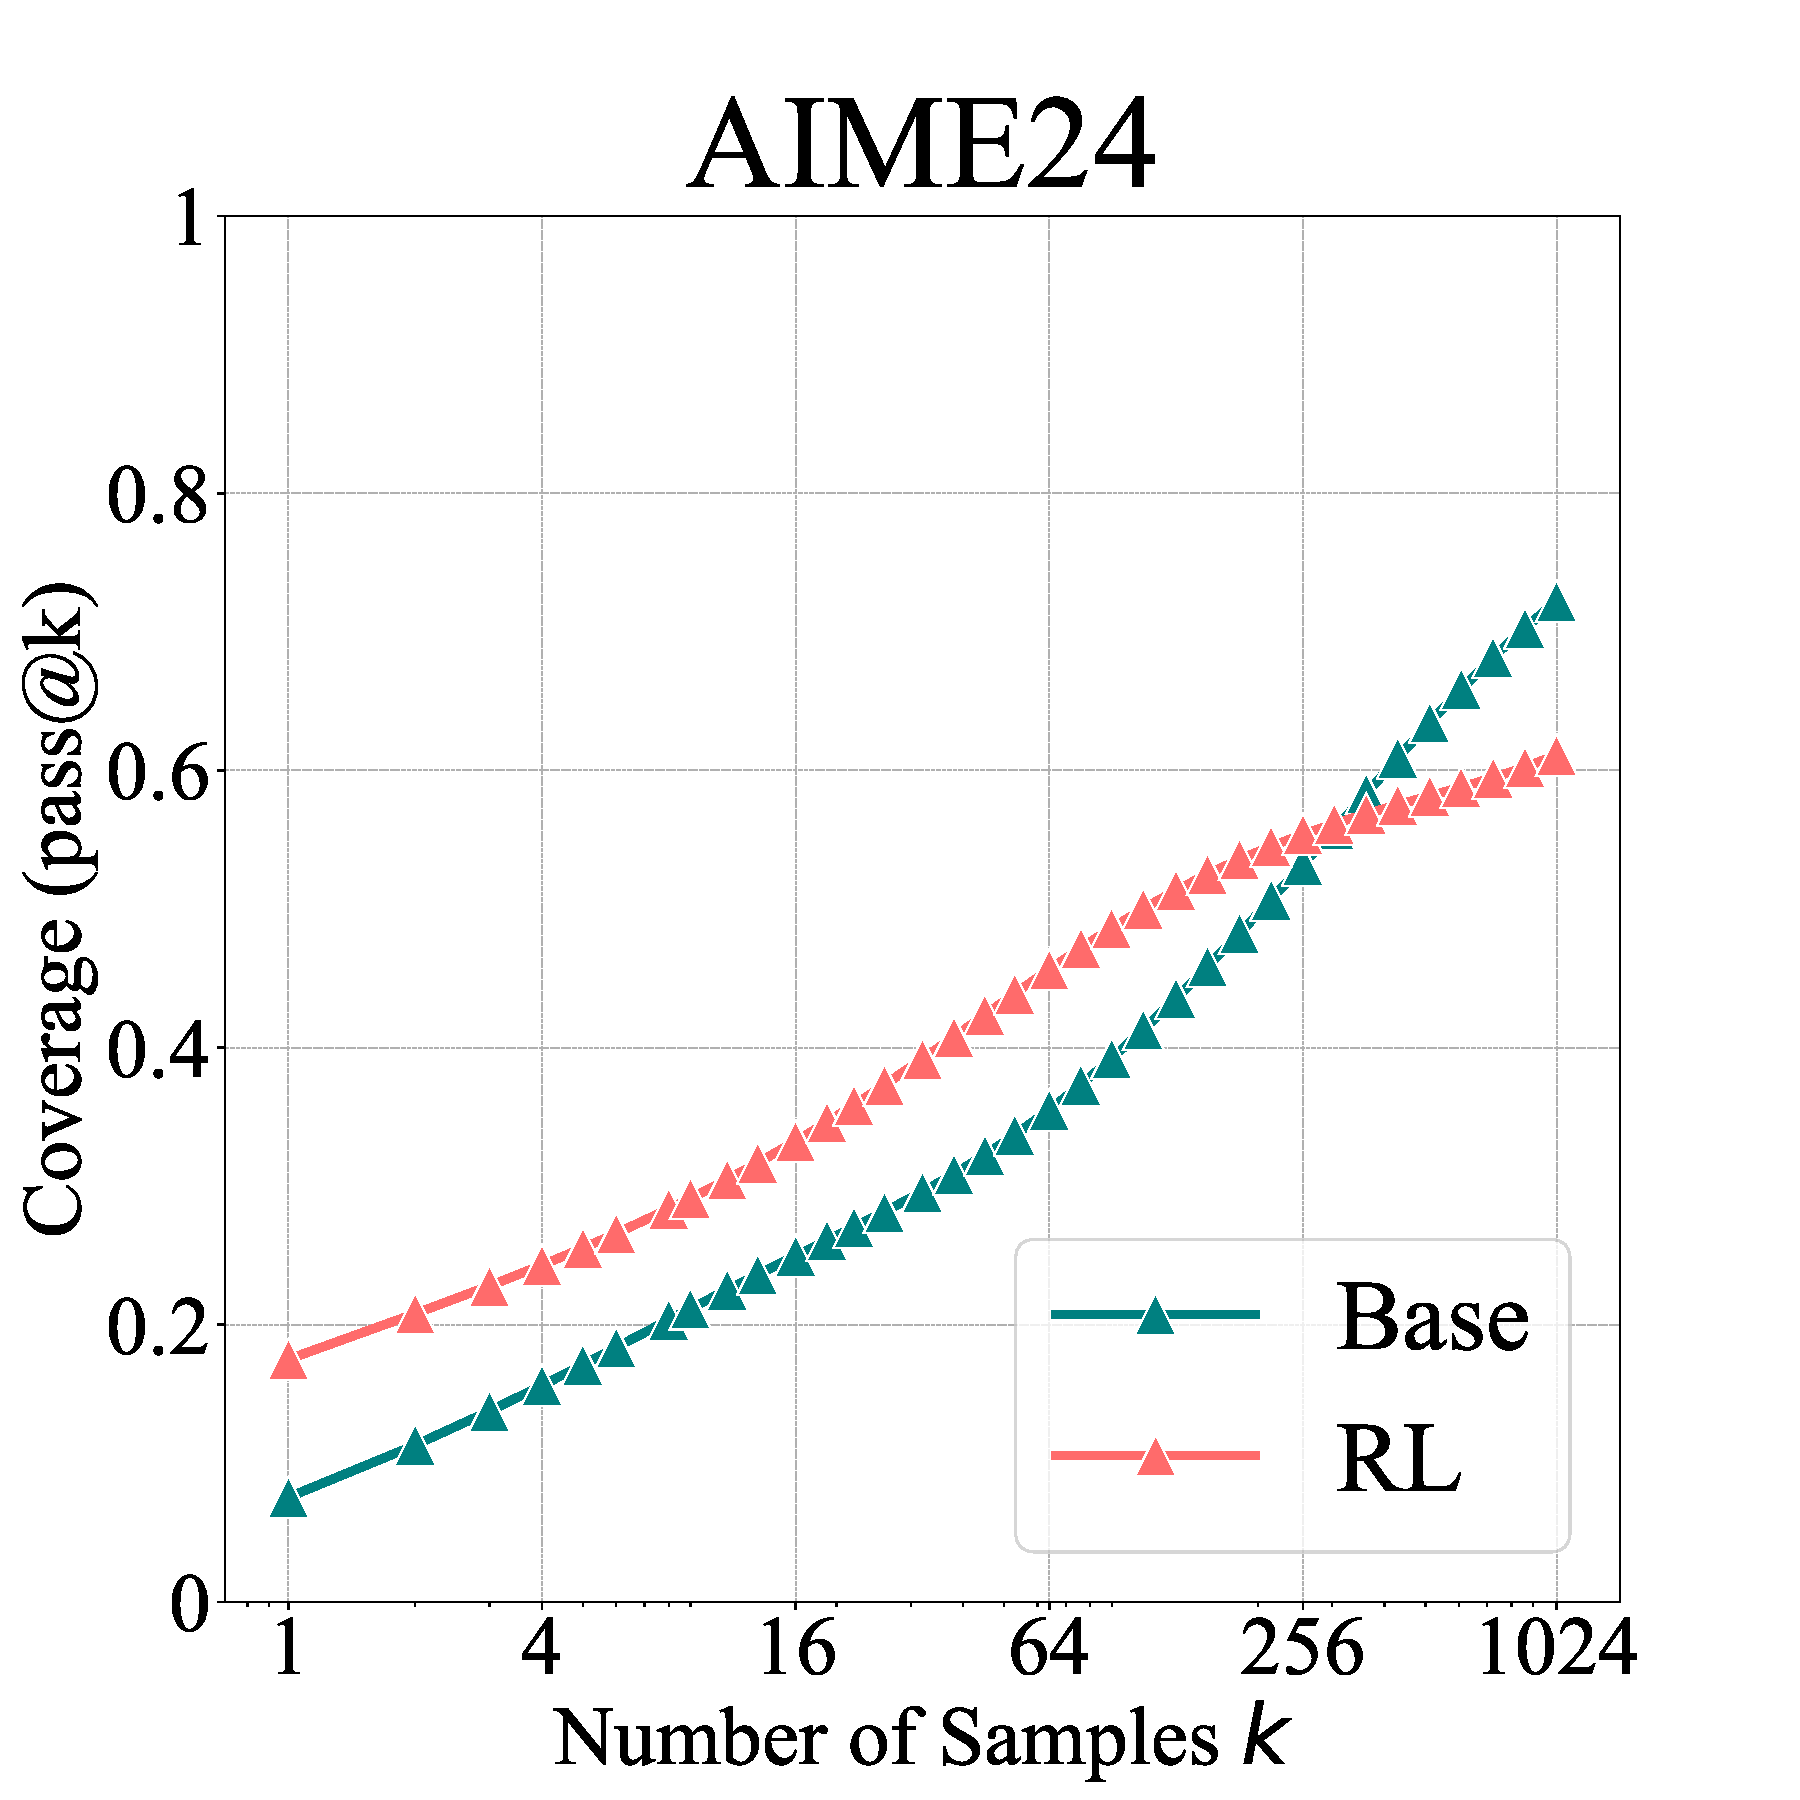
\includegraphics[width=\textwidth]{tex/images/simpleRL_coverage_aime24_filtered.pdf}
  \end{subfigure}
% \captionsetup{font={footnotesize}}
\vspace{-1mm}
\caption{
Pass@$k$ curves of the base and SimpleRLZoo-7B models in the filtered AIME24.
}
\label{fig:filtered_aime24}
\end{figure}

The base and RL model pass@$k$ curves on this filtered AIME24 can be found in~\cref{fig:filtered_aime24}, showing a similar trending to previous results. 
Although this filtering method is heuristic, it proves to be effective. 
Applying it to AIME24 (30 questions) results in a subset of 18 questions. We then prompt the models to answer these filtered questions using CoT reasoning.
Then we perform a manual inspection of all CoTs that led to correct answers on the hardest problems -- those with an average accuracy below 5\%. 
The base model answered 7 such questions, with 5 out of 6 containing \textit{at least one} correct CoT (excluding one ambiguous case of correctness due to skipped reasoning steps). Similarly, the RL-trained model answered 6 questions, 4 of which included \textit{at least one} correct CoT.
These results suggest that even for the hardest questions in the challenging AIME24, base model can sample valid reasoning paths to solve the problems.


\clearpage


\subsection{Accuracy Distribution Visulization}

\begin{figure}[H]
  \centering
   % \includegraphics[width=0.95\textwidth]{tex/images/simpleRL_coverage_verynew.pdf}
   \includegraphics[width=1.0\textwidth]{tex/images/simpleRL_his.pdf}
% \captionsetup{font={footnotesize}}
\caption{
Accuracy histogram before and after RLVR with SimpleRLZoo models.
}
\label{fig:hist_all}
\vspace{-5mm}
\end{figure}


\clearpage
\subsection{Perplexity Analysis}
\label{appendix:perplexity}

To analyze how perplexity evolves over the course of RLVR training, we evaluated three RLVR checkpoints--early, middle, and final in~\cref{sec:algos} RL training. For each checkpoint, we sampled 32 responses per problem, computed the median among 32 perplexity values, and reported the average over the first 10 problems in the table.
As expected, we observed that $\text{PPL}_\text{Base} (\mathbf{Y}_\text{RL} | x)$ gradually decreases as RL training progresses, indicating that RLVR mainly sharpens the distribution within the base model's prior rather than expanding beyond it.

\begin{figure}[!h]
\vspace{-3mm}
  \centering
  \begin{subfigure}[b]{0.5\textwidth}
    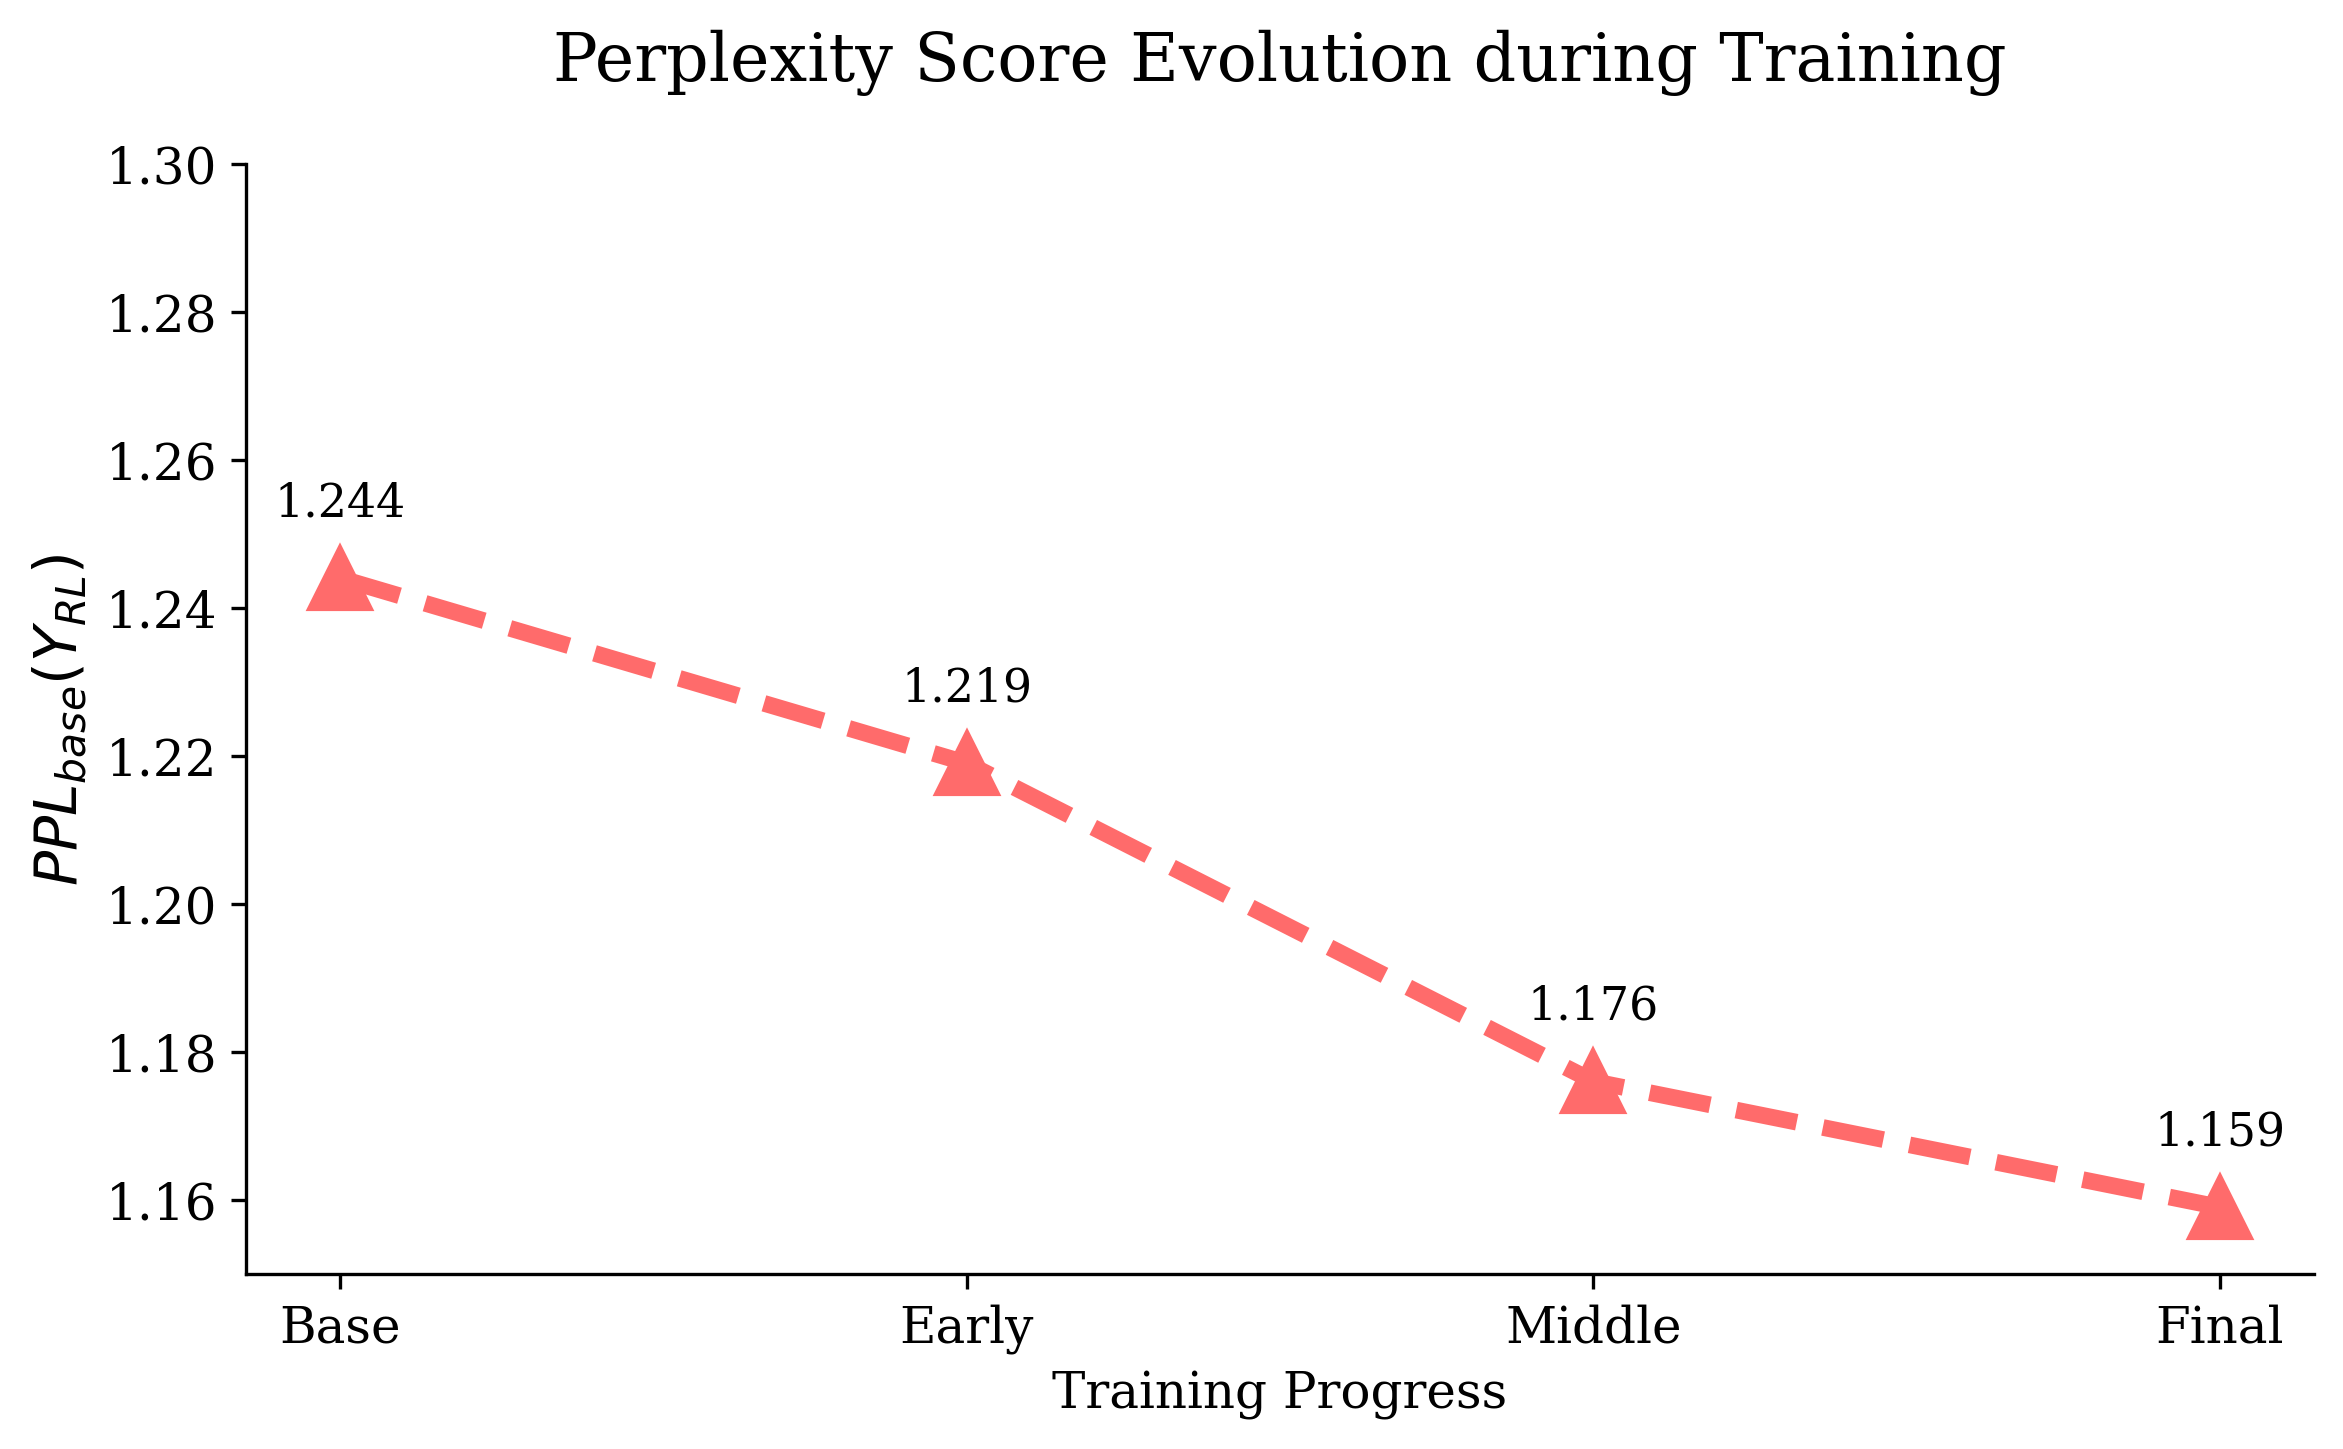
\includegraphics[width=\textwidth]{tex/images/perplexity_time.png}
  \end{subfigure}
\caption{
Perplexity Evolution during RL Training.
}
\label{fig:perplexity_time}
\vspace{-3mm}
\end{figure}

\subsection{Different RLVR Algorithms}
\label{appendix:algos}

We report several additional observations on different RLVR algorithms in~\cref{fig:algo_and_step}. First, DAPO achieves slightly higher pass@1 scores across all three datasets; however, its dynamic sampling strategy requires approximately $3 \sim 6\times$ more samples per batch during training compared to other algorithms. Moreover, its performance drops significantly at $k = 256$.
Second, RLOO and Reinforce++ perform consistently well across the entire $k$ range (from 1 to 256), while maintaining efficient training costs, achieving a good balance between effectiveness and efficiency.
Third, ReMax shows lower performance at both pass@1 and pass@256. We hypothesize that this is due to its use of the greedy response reward as the advantage baseline, which in the RLVR setting is binary (0 or 1) and highly variable. This likely results in unstable gradient updates during training.

\begin{table}[H]
\vspace{-2mm}
\centering
\caption{Detailed values for each point at pass@1 and pass@256 across different RL algorithms in~\cref{fig:algo_and_step}.}
\label{tab:algos}
\resizebox{0.65\textwidth}{!}{
\begin{tabular}{l|cc|cc|cc}
\toprule
\textbf{Model} &
\multicolumn{2}{c|}{\textbf{Omni-MATH-Train}} &
\multicolumn{2}{c|}{\textbf{Omni-MATH-Test}} &
\multicolumn{2}{c}{\textbf{MATH500}} \\
 & pass@1 & pass@256 & pass@1 & pass@256 & pass@1 & pass@256 \\
\midrule
Qwen2.5-7B   & 9.9 & 67.2 & 10.2 & 69.1 & 34.5 & 96.2 \\
GRPO         & 26.1 & 66.3 & 25.1 & 68.3 & 74.4 & 97.2 \\
PPO          & 27.2 & 65.8 & 26.8 & 69.2 & 75.2 & 97.2 \\
ReMax        & 24.4 & 65.5 & 23.8 & 67.5 & 73.5 & 96.6 \\
RLOO         & 28.6 & 66.4 & \textbf{28.1} & 69.2 & 75.0 & \textbf{97.4} \\
Reinforce++  & 28.2 & \textbf{67.7} & \textbf{28.0} & \textbf{69.7} & 75.4 & 96.8 \\
DAPO         & \textbf{31.4} & 66.1 & 26.5 & 67.0 & \textbf{75.6} & 96.4 \\
\bottomrule
\end{tabular}
}
% \vspace{-2mm}
\end{table}

\begin{table}[H]
\vspace{-2mm}
\centering
\caption{Detailed values at pass@1 and pass@256 across different RL training steps in~\cref{fig:overview} (right).}
\label{tab:grpo_training_steps}
\resizebox{0.65\textwidth}{!}{
\begin{tabular}{l|cc|cc|cc}
\toprule
\textbf{Model} &
\multicolumn{2}{c|}{\textbf{Omni-MATH-Train}} &
\multicolumn{2}{c|}{\textbf{Omni-MATH-Test}} &
\multicolumn{2}{c}{\textbf{MATH500}} \\
 & pass@1 & pass@256 & pass@1 & pass@256 & pass@1 & pass@256 \\
\midrule
Qwen2.5-7B       & 9.9 & \textbf{67.2} & 10.2 & \textbf{69.1} & 34.5 & 96.2 \\
GRPO-step150     & 26.1 & 66.3 & 25.1 & 68.3 & 74.4 & \textbf{97.2} \\
GRPO-step300     & 33.6 & 65.3 & 27.1 & 66.6 & 75.4 & 96.0 \\
GRPO-step450     & \textbf{42.5} & 64.3 & \textbf{28.3} & 63.9 & \textbf{76.3} & 95.4 \\
\bottomrule
\end{tabular}
}
\vspace{-2mm}
\end{table}



\vspace{1mm}

\clearpage
\subsection{Effects of KL and Rollout Number}

\begin{figure}[!h]
  \centering
  \begin{subfigure}[b]{0.98\textwidth}
    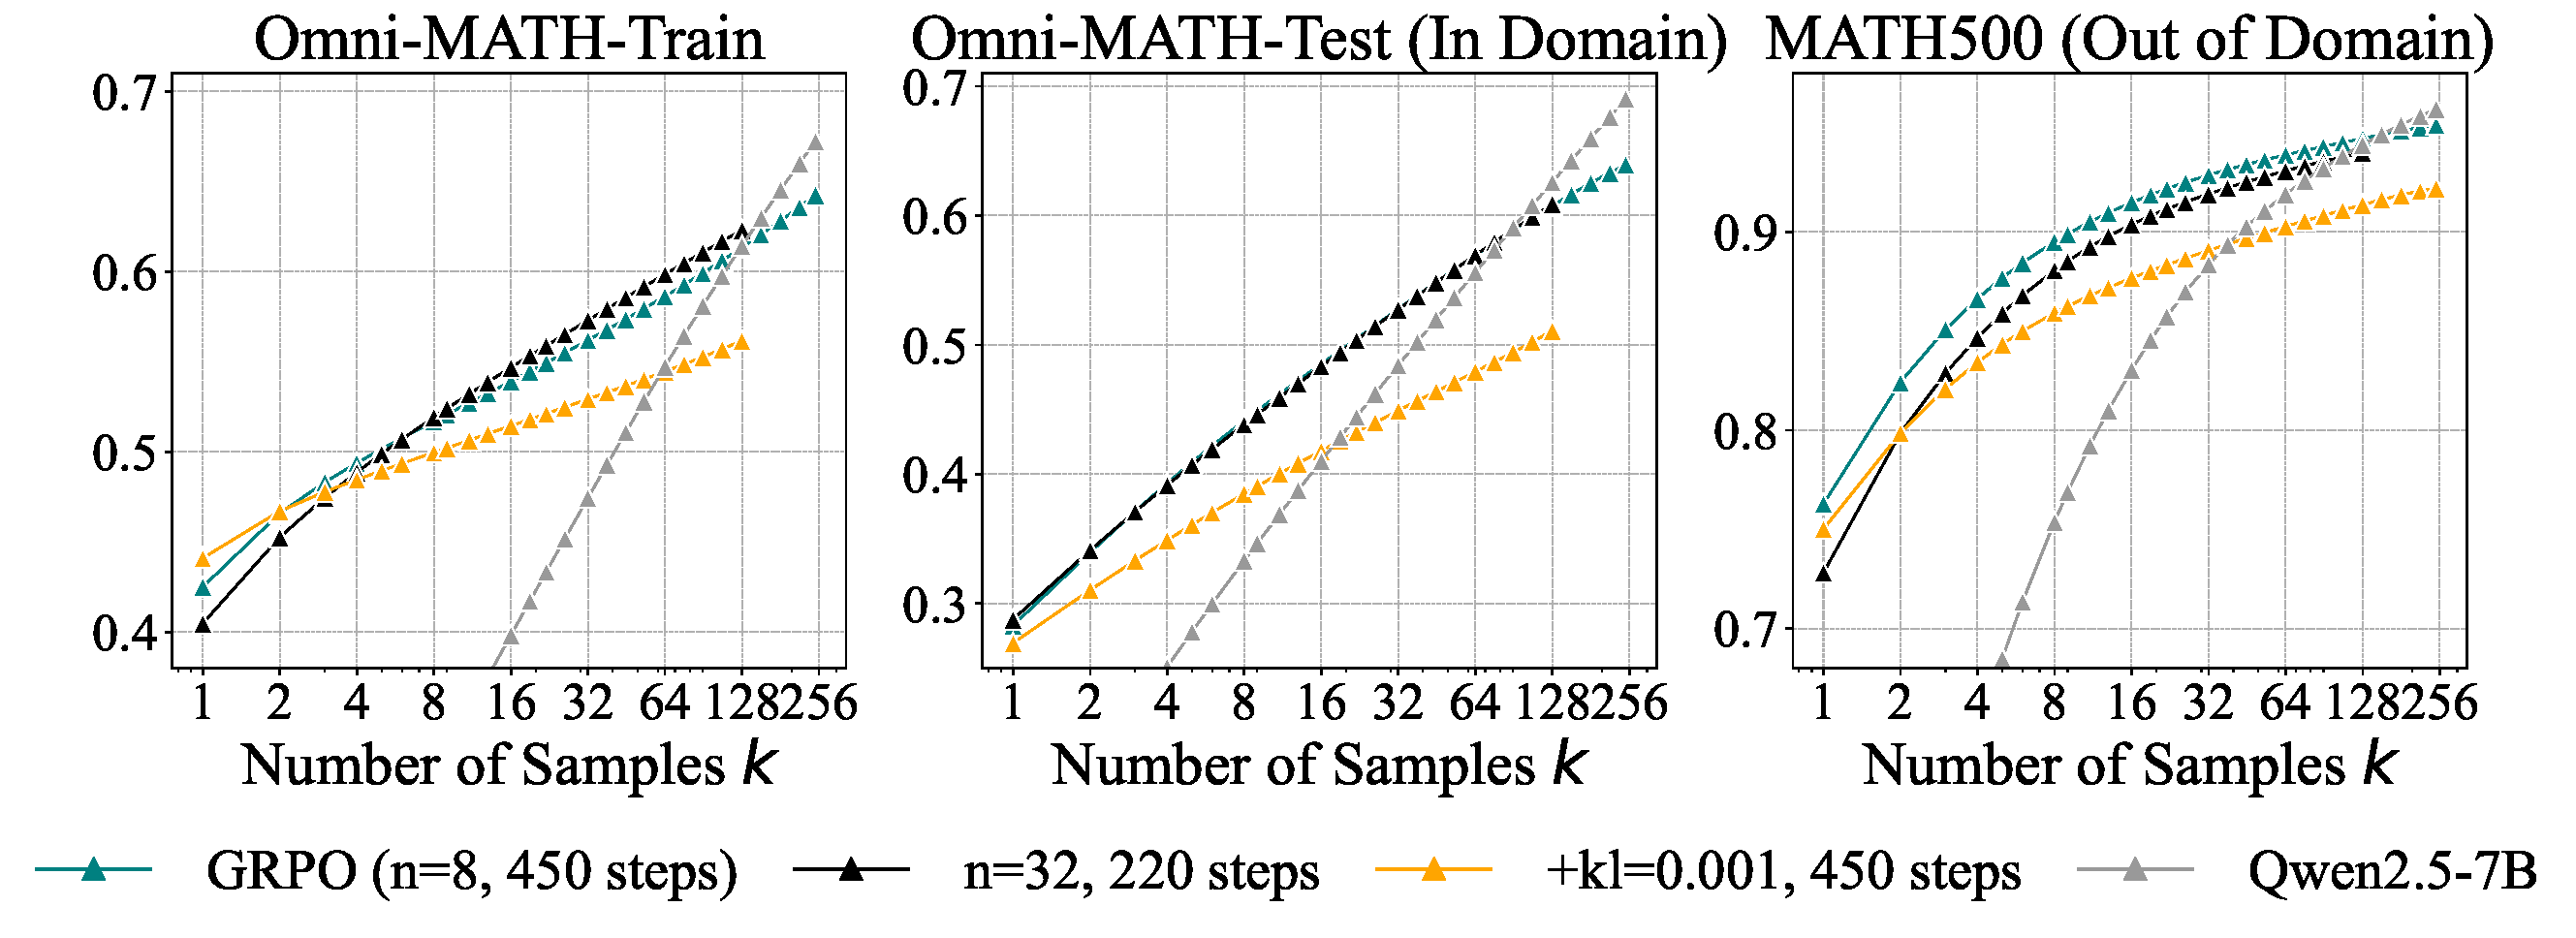
\includegraphics[width=\textwidth]{tex/images/qwen25_7b_base_ablate_coverage.pdf}
  \end{subfigure}
\caption{
\textbf{
Ablation Study on KL Loss and Rollout Number $n$.}
For increasing $n$ from 8 to 32, we keep the prompt batch size unchanged, which results in increased computation per training step. 
Due to resource constraints, we train for only 220 steps under this setting, leading to lower pass@1 as the model has not yet converged. 
Nevertheless, the model with $n = 32$ achieves a higher pass@128, highlighting the positive effect of larger rollout numbers in improving pass@$k$ at higher values of $k$.
}
\label{fig:grpo_ablate}
% \vspace{-3mm}
\end{figure}



\subsection{Solvable Problem Coverage Analysis}
\label{app:coverage_analysis}

\cref{tab:four_categories} reports the fraction of problems categorized as four conditions: (1) both models solve the problem at least once, (2) only the base model solves it, (3) only the RLVR model solves it, and (4) neither model solves it in any of the $k$ samples. 
It highlights that there are many cases where the base model solves a problem but RLVR fails (type 2), and very few where RLVR succeeds while the base does not (type 3). Even in the rare type 3 cases (e.g., 1\% or about 5 problems in MATH500), the base model is able to solve all of them when sampling 1024 times. These results support our conclusion that RLVR rarely solves problems the base model cannot and generally results in reduced coverage.


\begin{table}[!h]
\centering
\caption{Indices of solvable problems in AIME24 (starting from 0). An approximate subset relationship can be observed: most problems solved by the RL model are also solvable by the base model.}
\label{tab:sovable_aime24}
\resizebox{0.9\textwidth}{!}{
\begin{tabular}{cc}
\toprule
\textbf{Models} & \textbf{Problem Indices} \\
\midrule
Qwen2.5-7B-Base & 0, 1, 4, 6, 7, 8, 9, 11, 12, 14, 15, 16, 17, 18, 19, 22, 23, 24, 25, 26, 27, 28, 29 \\
\midrule
SimpleRL-Qwen2.5-7B & 0, 1, 6, 7, 8, 9, 12, 14, 15, 16, 18, 22, 23, 24, 25, 26, 27, 28, 29 \\
\bottomrule
\end{tabular}
}
% \vspace{4mm}
\end{table}



\begin{table}[!h]
\centering
\caption{Indices of solvable problems in LiveCodeBench (ranging from 400 to 450, starting from 0). }
\label{tab:solvable_livecodebench}
\resizebox{0.7\textwidth}{!}{
\begin{tabular}{cc}
\toprule
\textbf{Model} & \textbf{Solvable Problem Indices} \\
\midrule
Qwen2.5-7B-Instruct-1M & 
\makecell[c]{400, 402, 403, 407, 409, 412, 413, 417, 418, 419, 422, 423, \\427, 432, 433, 436, 438, 439, 440, 444, 445, 448, 449} \\
\midrule
Coder-R1 & 
\makecell[c]{400, 402, 403, 407, 412, 413, 417, 418, 419, 422, 423, \\427, 430, 433, 438, 439, 440, 444, 445, 449} \\
\bottomrule
\end{tabular}
}
\vspace{-3mm}
\end{table}


\vspace{1mm}


\clearpage
\subsection{Temperature and Entropy Analysis}

\begin{figure}[h]
\vspace{-3mm}
  \centering
  \begin{subfigure}[b]{0.6\textwidth}
    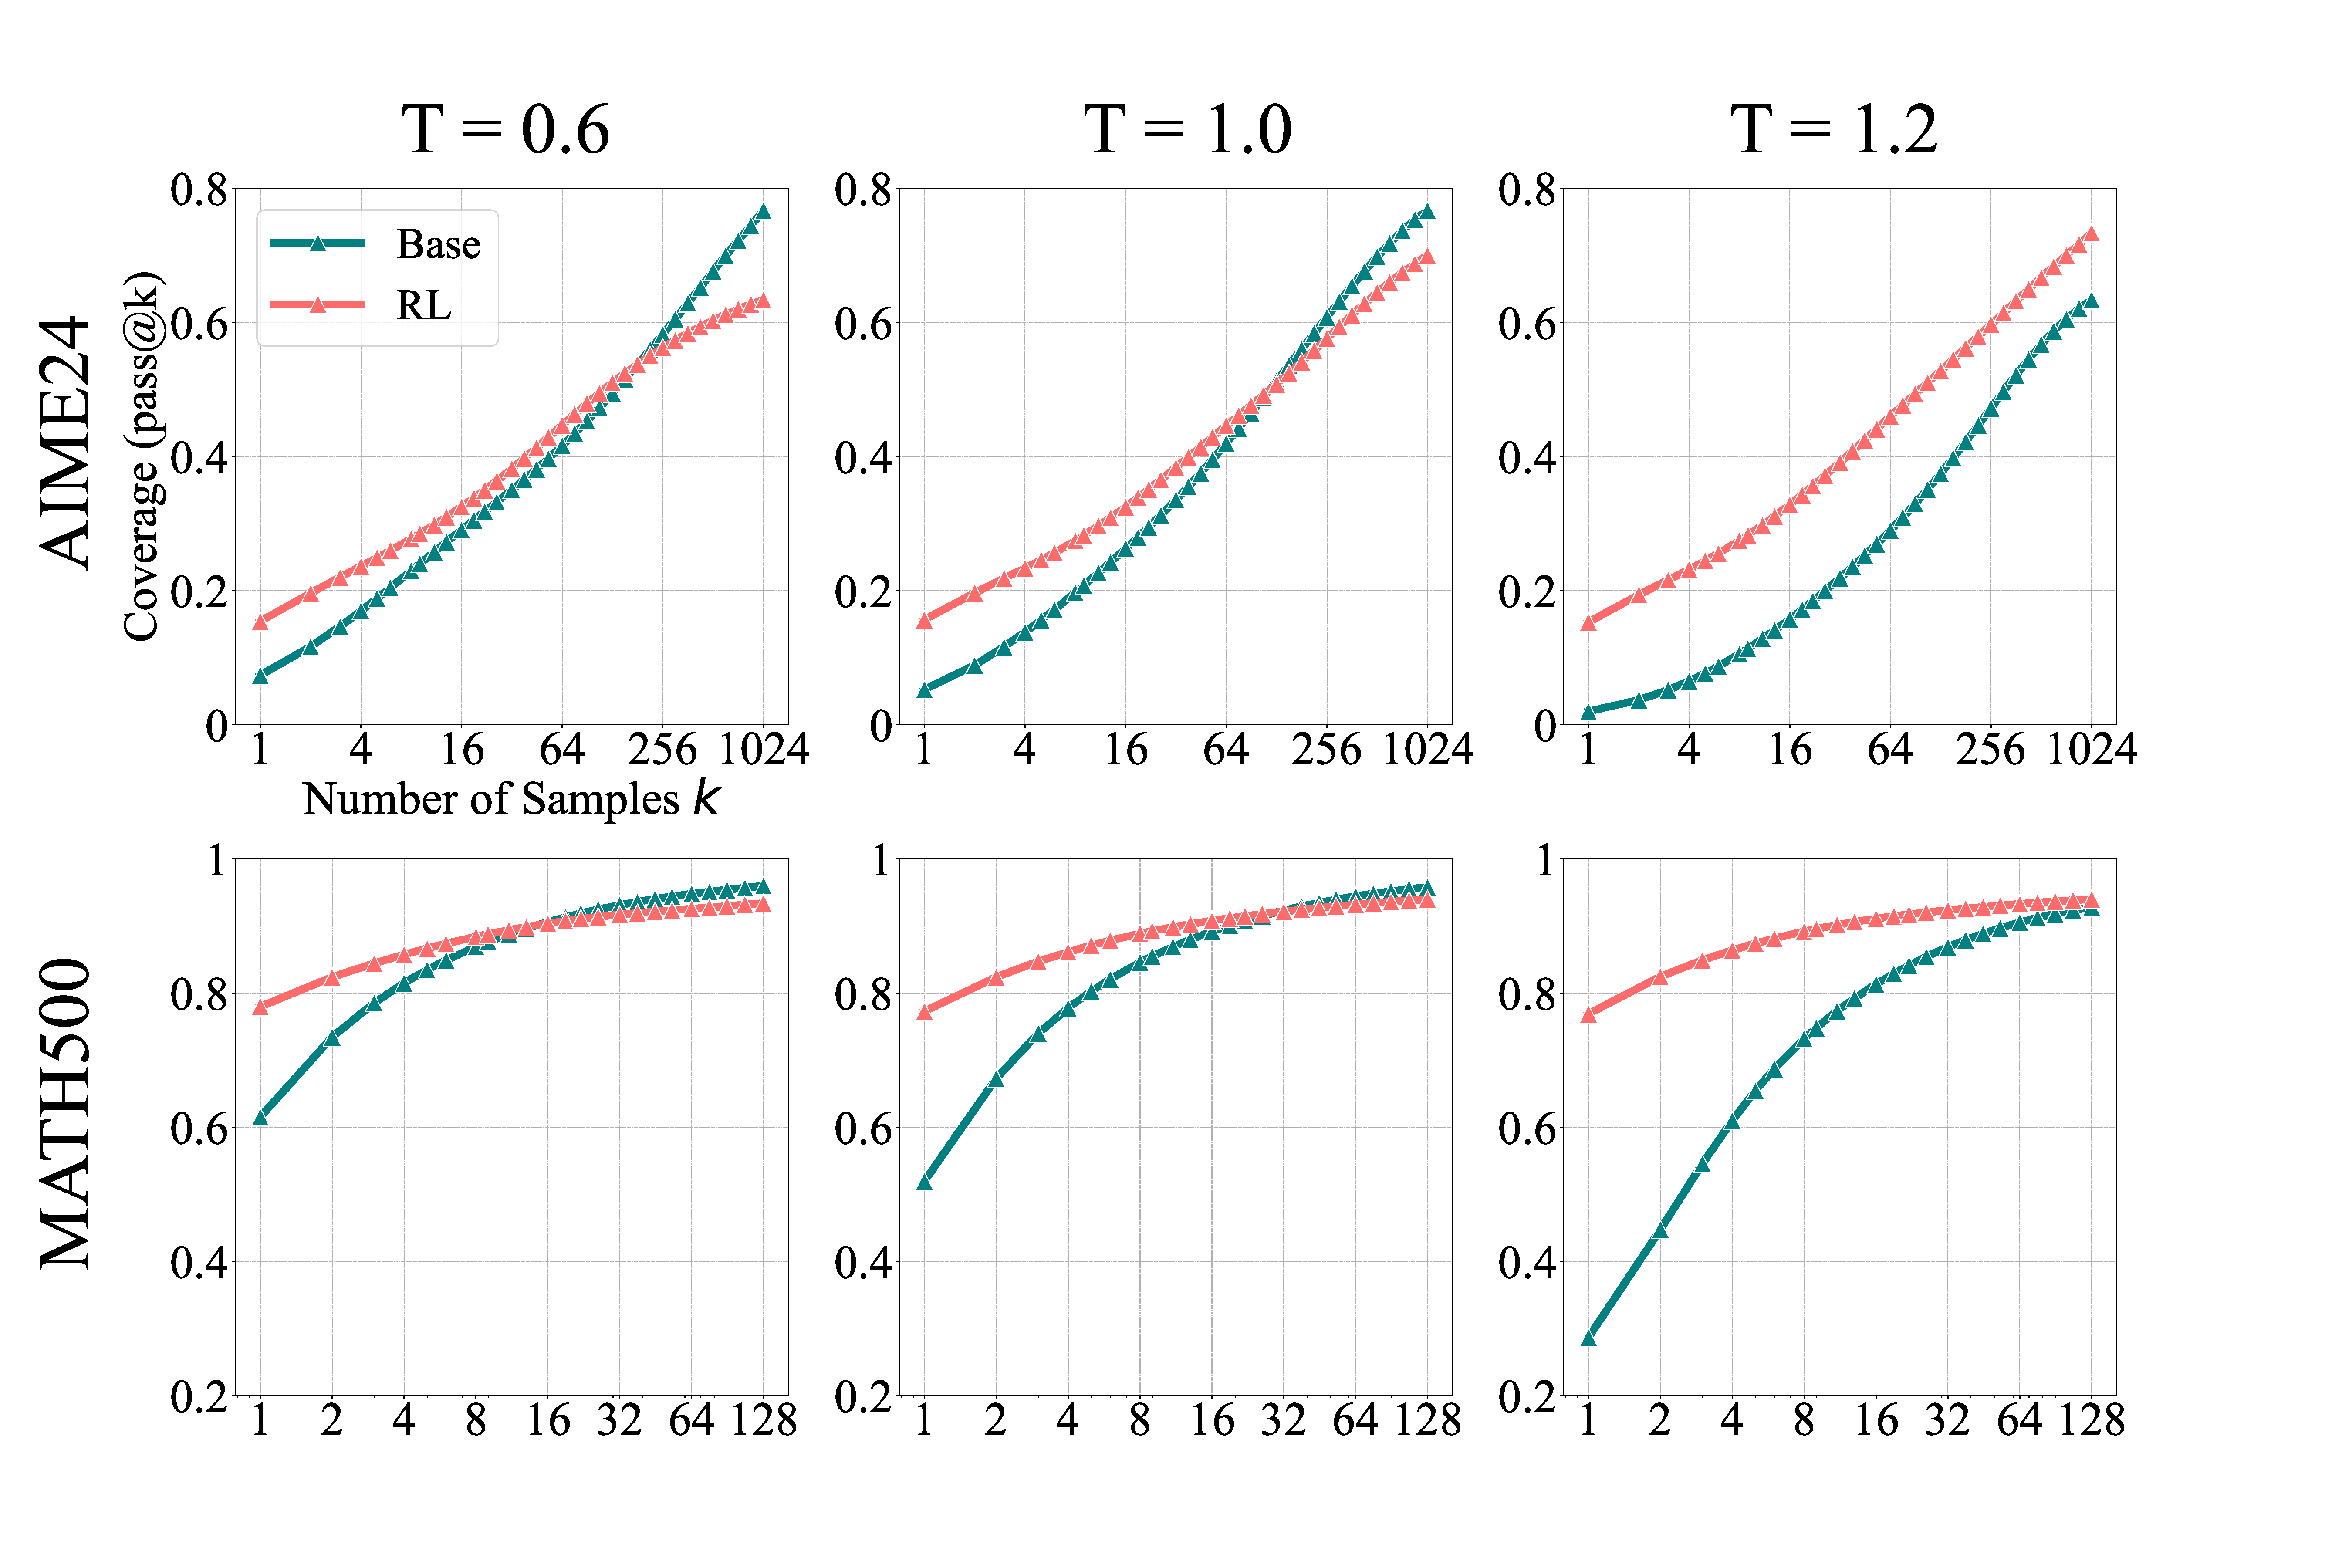
\includegraphics[width=\textwidth]{tex/images/simpleRL_coverage_difT.pdf}
  \end{subfigure}
\captionsetup{font={footnotesize}}
\caption{
We found that the base model's performance drops when the temperature exceeds 1.0, as it tends to generate more random and less coherent tokens. In contrast, the RL model's performance remains relatively stable across different temperature settings. Therefore, we use $T = 0.6$ in the main experiments, as it allows both models to demonstrate their best reasoning performance.
}
\label{fig:different_T}
\vspace{-3mm}
\end{figure}


\begin{figure}[h]
\vspace{-3mm}
  \centering
  \begin{subfigure}[b]{0.65\textwidth}
    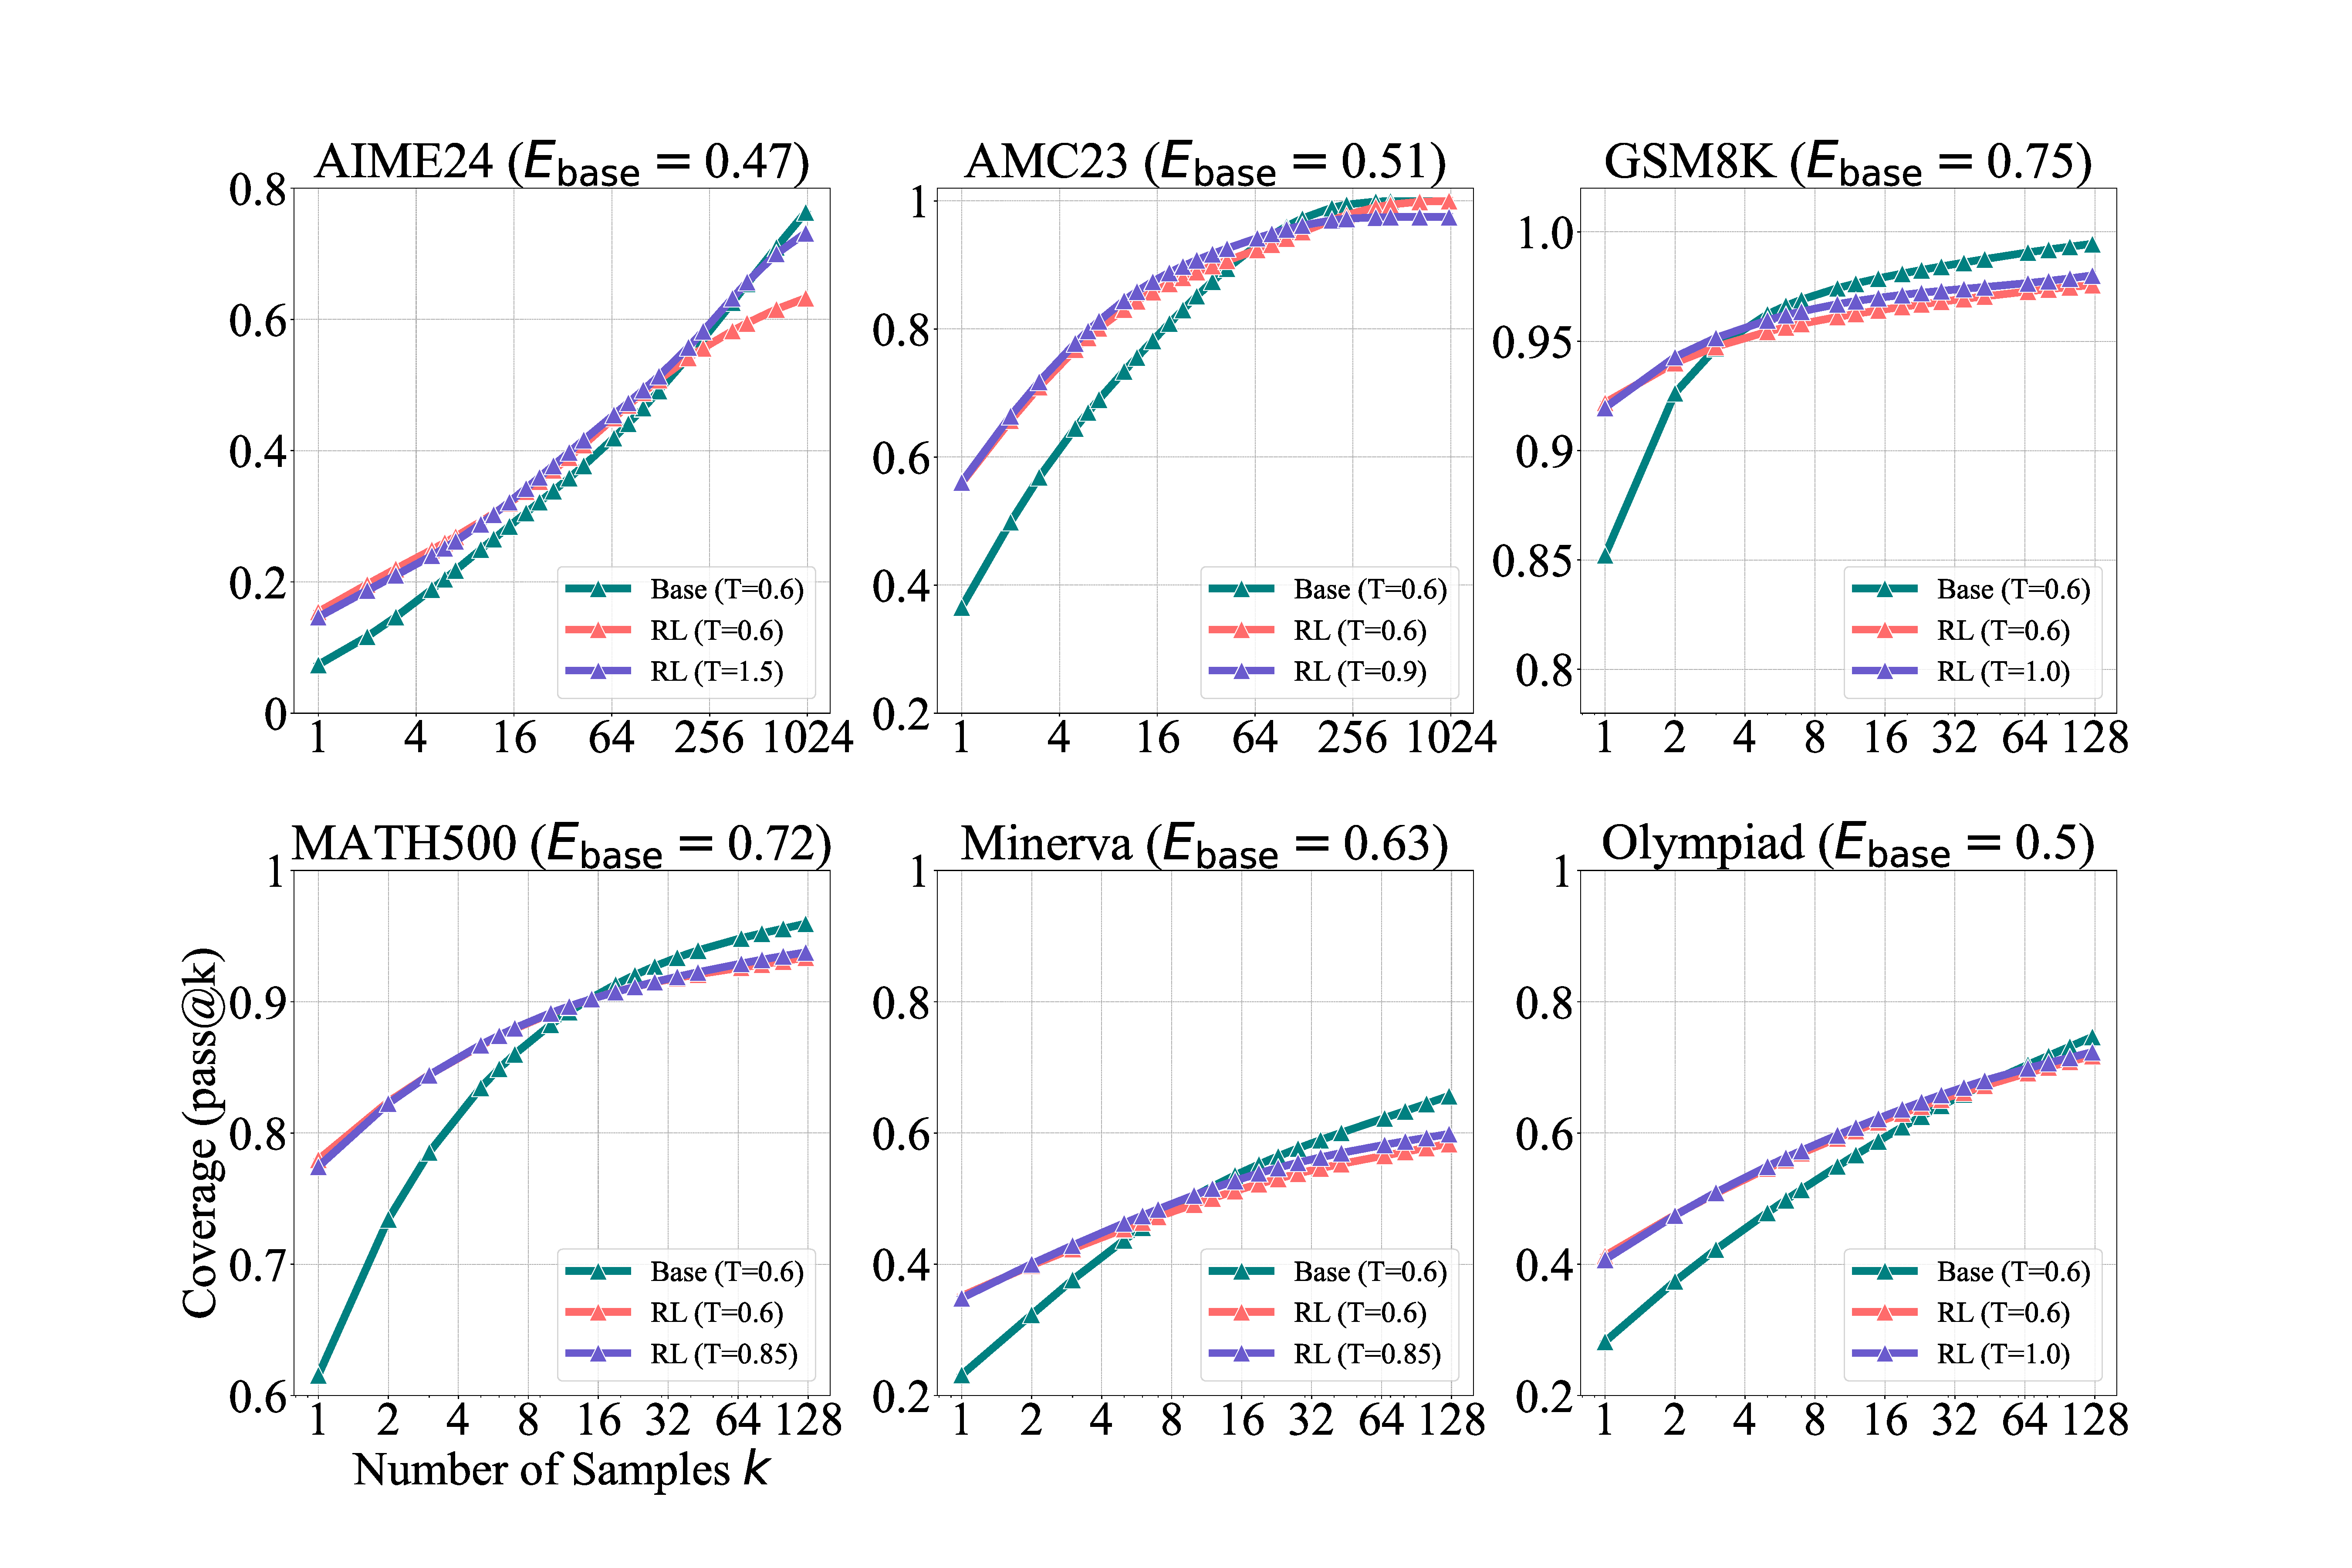
\includegraphics[width=\textwidth]{tex/images/simpleRL_coverage_entropy_T.pdf}
  \end{subfigure}
\captionsetup{font={footnotesize}}
\caption{
\textbf{Comparison of Base and RLVR Models with Matched Output Entropy.}
We evaluate the base model (Qwen2.5-7B) on each dataset using temperature $T=0.6$ and report its output entropy $E_\text{base}$ in the title of each figure. 
To enable a fair comparison, we increase the temperature of the RLVR model (SimpleRLZoo) until its output entropy approximately matches $E_\text{base}$. For example, on AMC23, we set $T=0.9$ to achieve $E_\text{RL} = 0.47$. 
We also include RLVR results at $T=0.6$ as an additional baseline, which has lower entropy---e.g., 0.22 on AMC23 and 0.33 on MATH500.
}
\label{fig:equal_entropy}
\vspace{-5mm}
\end{figure}

\clearpage
\subsection{Training Dynamics}

\begin{figure}[H]
\vspace{-3mm}
  \centering
  \begin{subfigure}[b]{0.68\textwidth}
    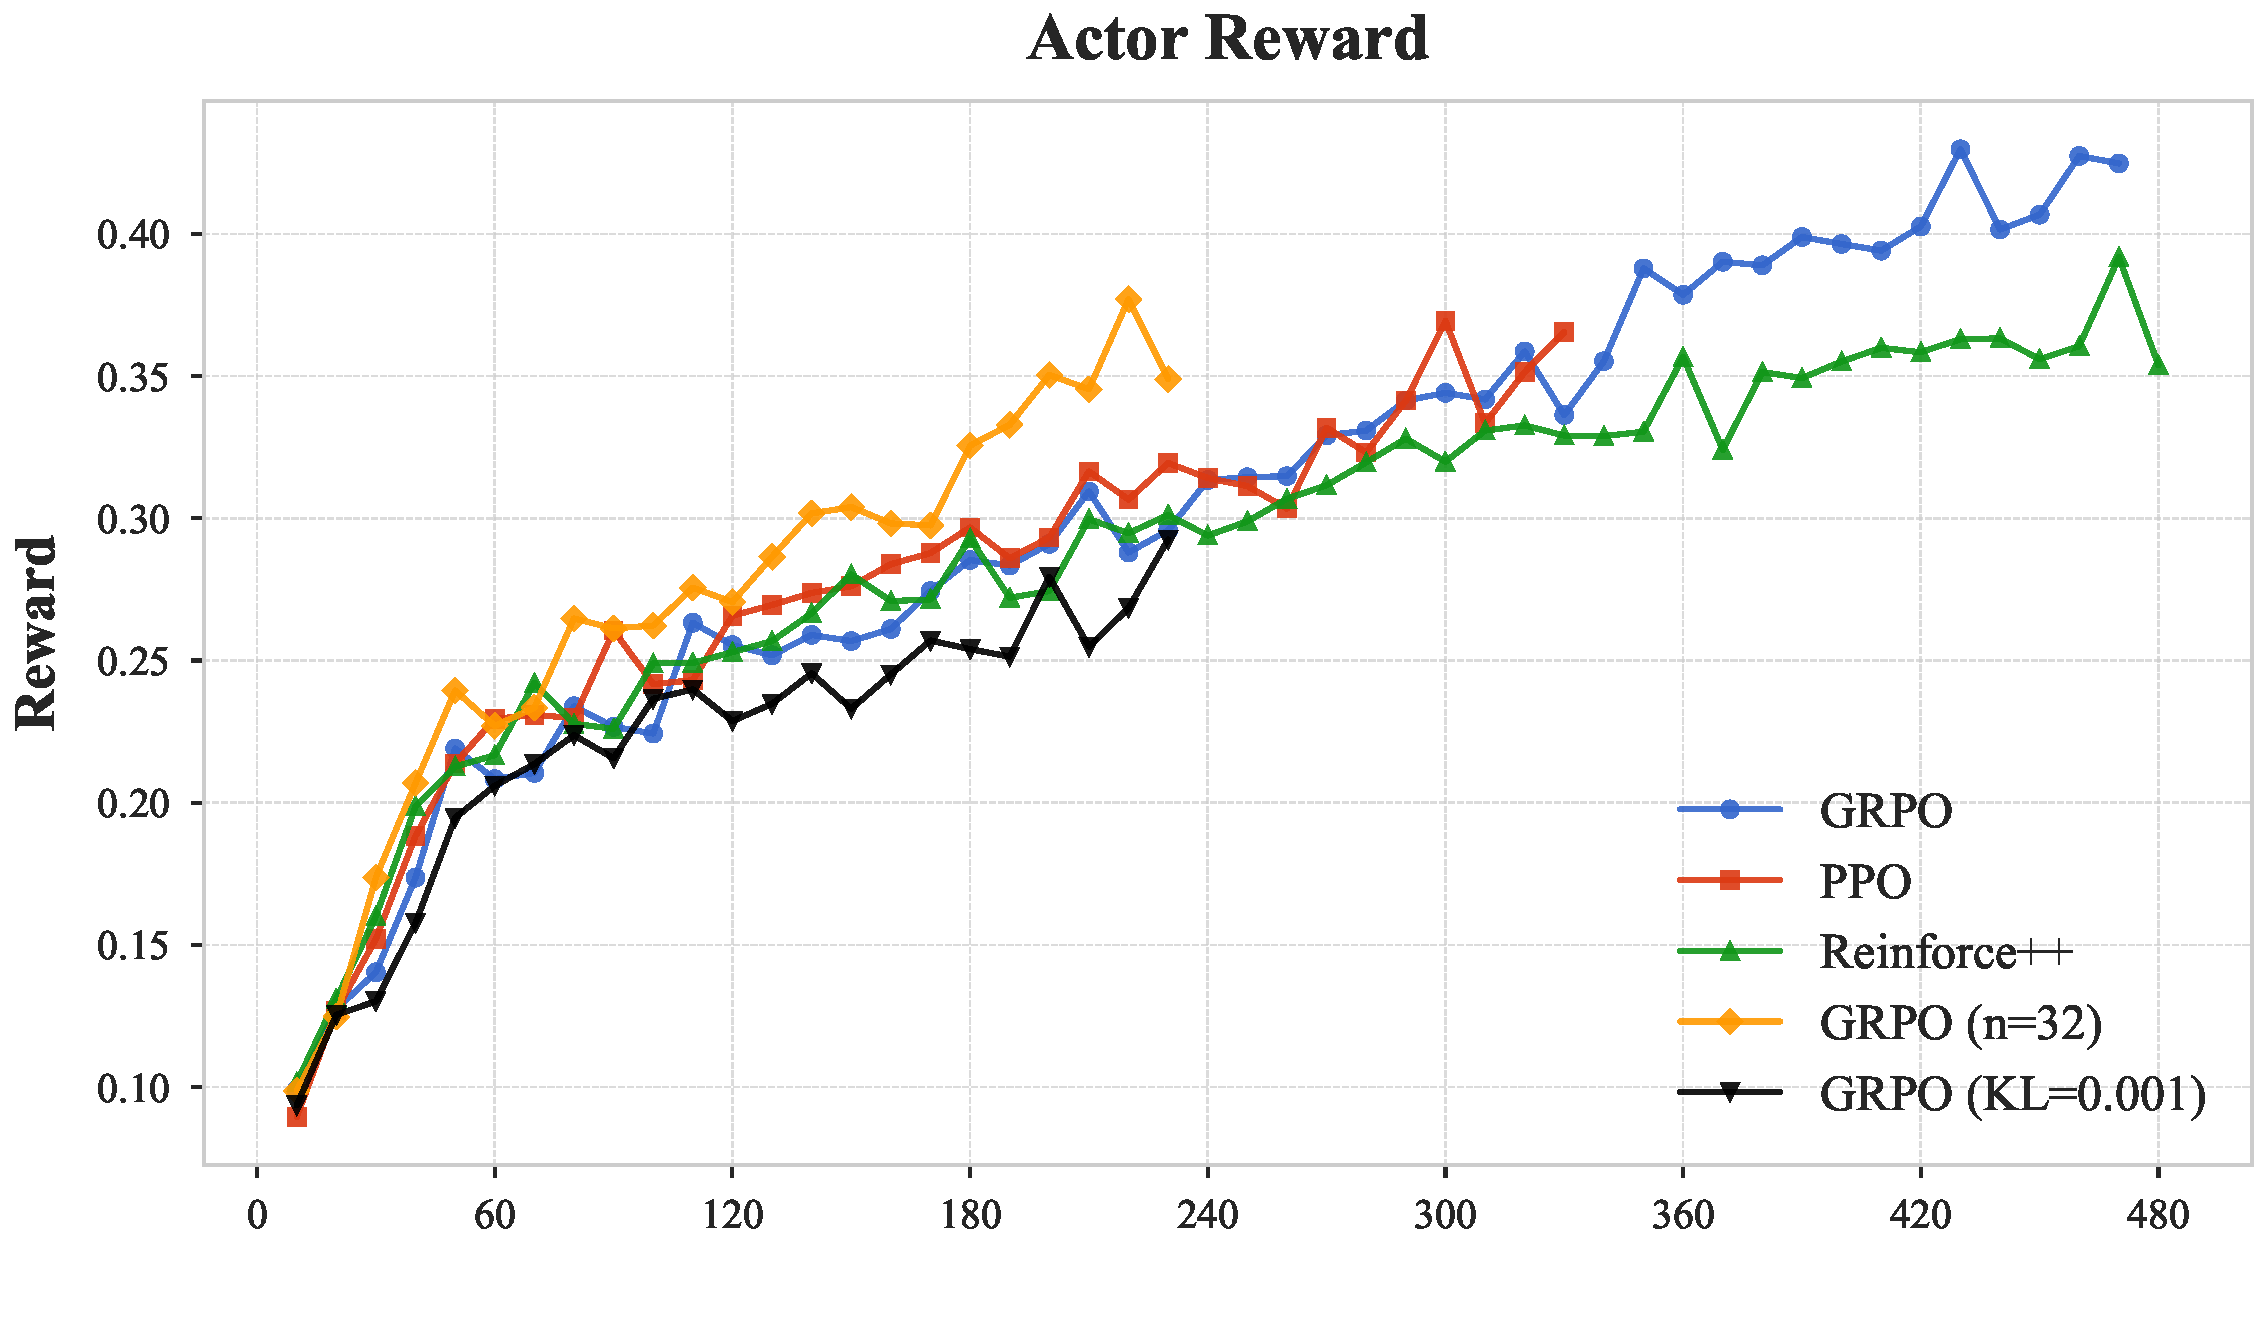
\includegraphics[width=\textwidth]{tex/images/dynamics_reward.pdf}
  \end{subfigure}
  \begin{subfigure}[b]{0.68\textwidth}
    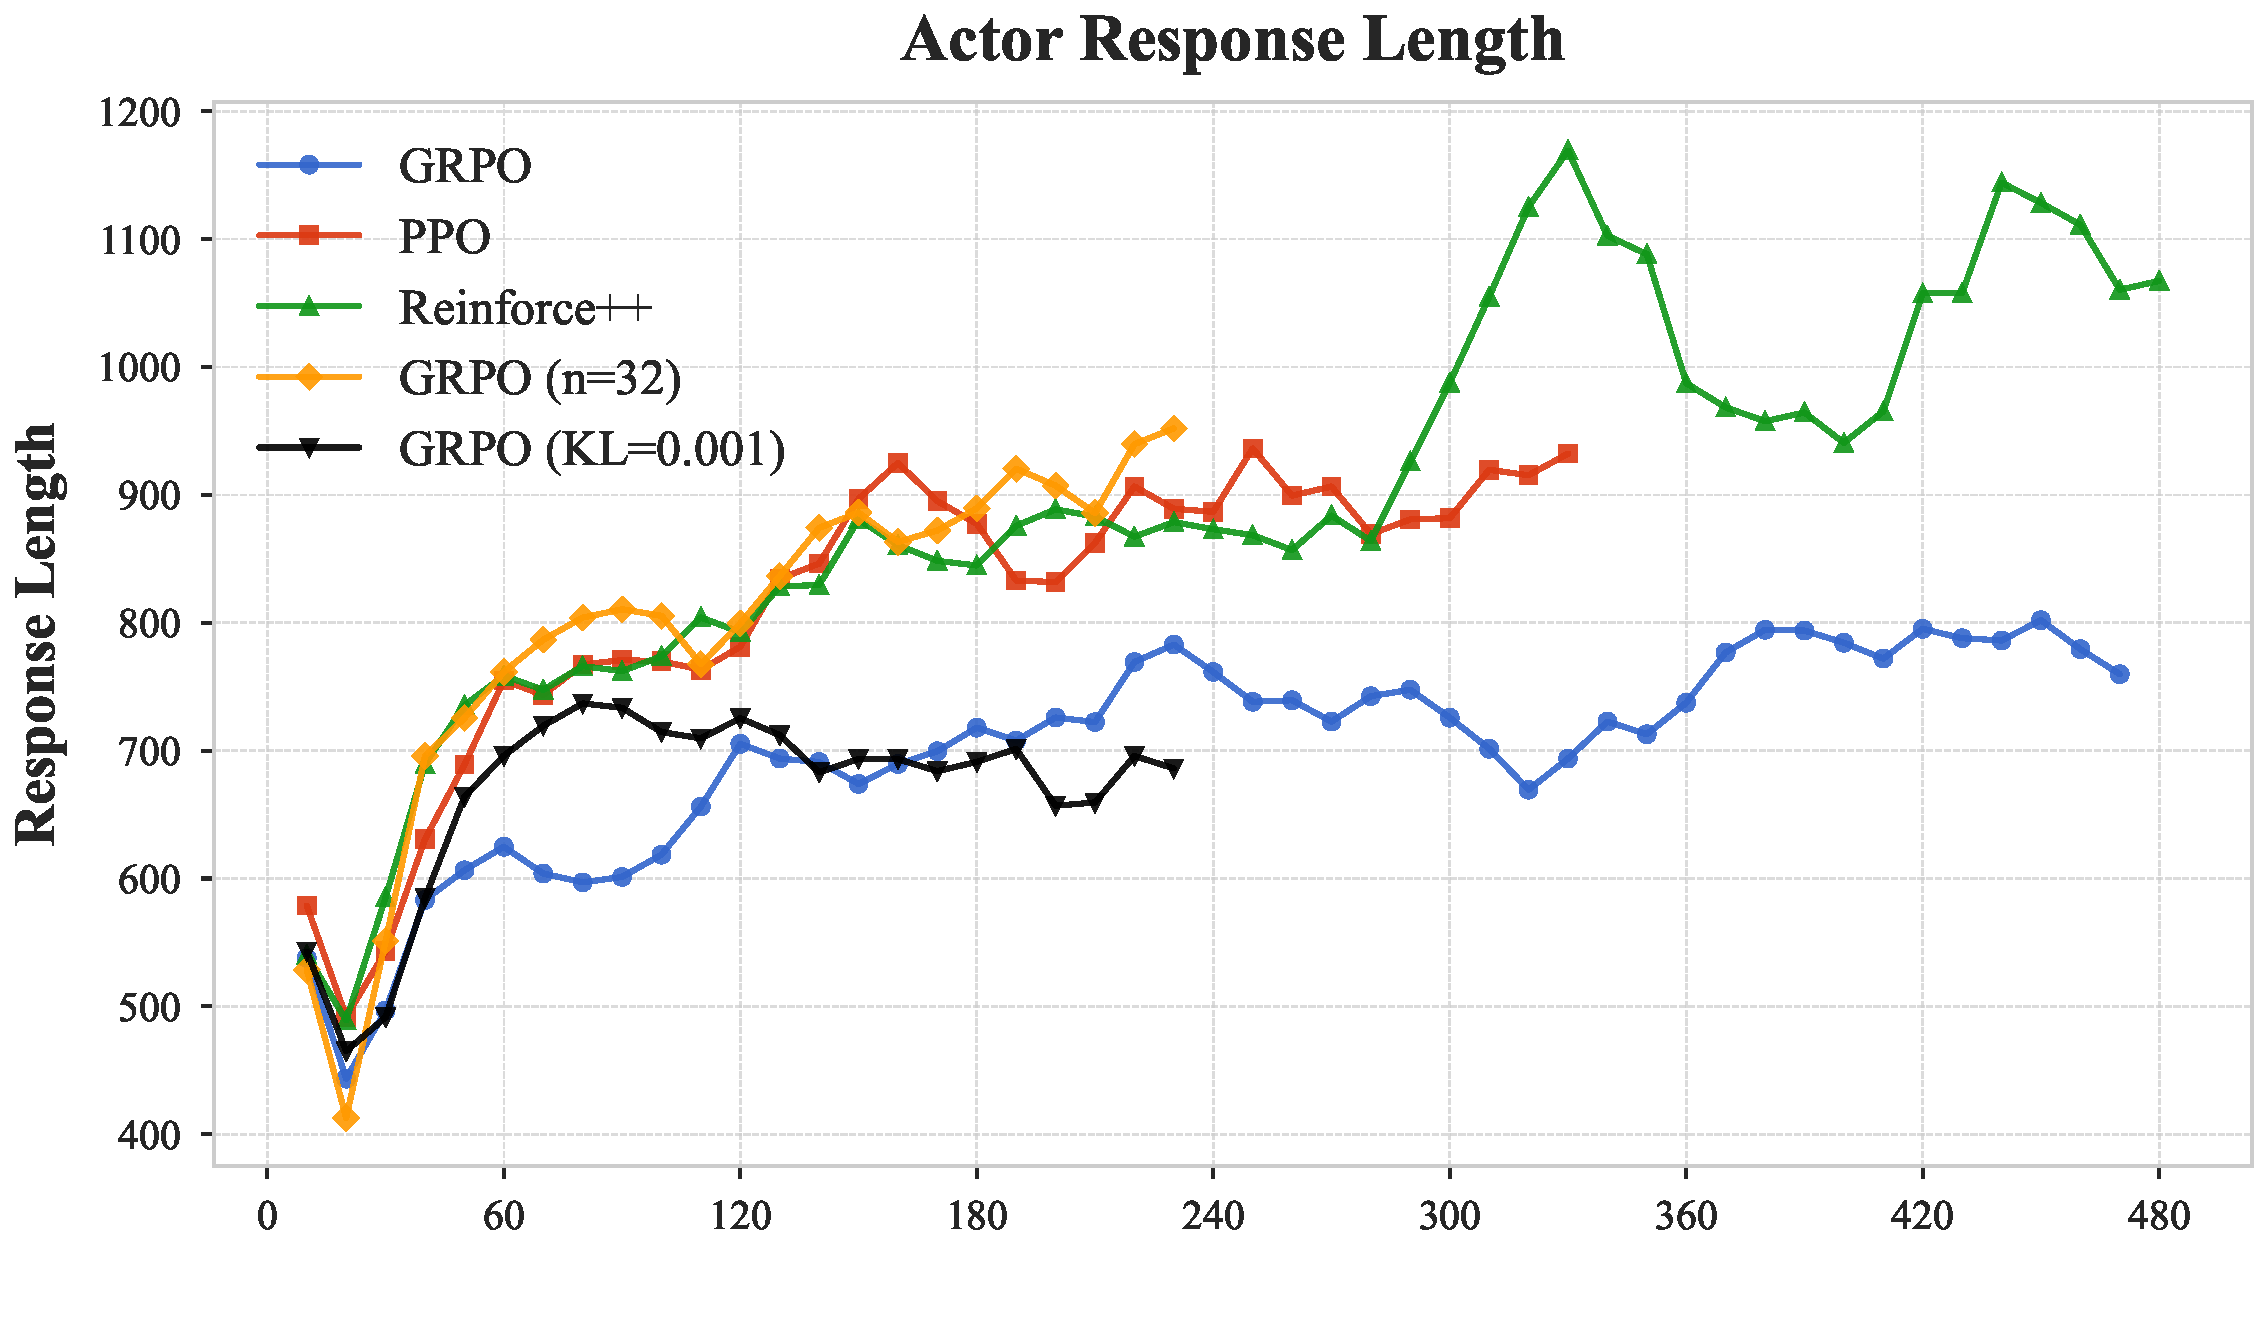
\includegraphics[width=\textwidth]{tex/images/dynamics_response_length.pdf}
  \end{subfigure}
\begin{subfigure}[b]{0.68\textwidth}
    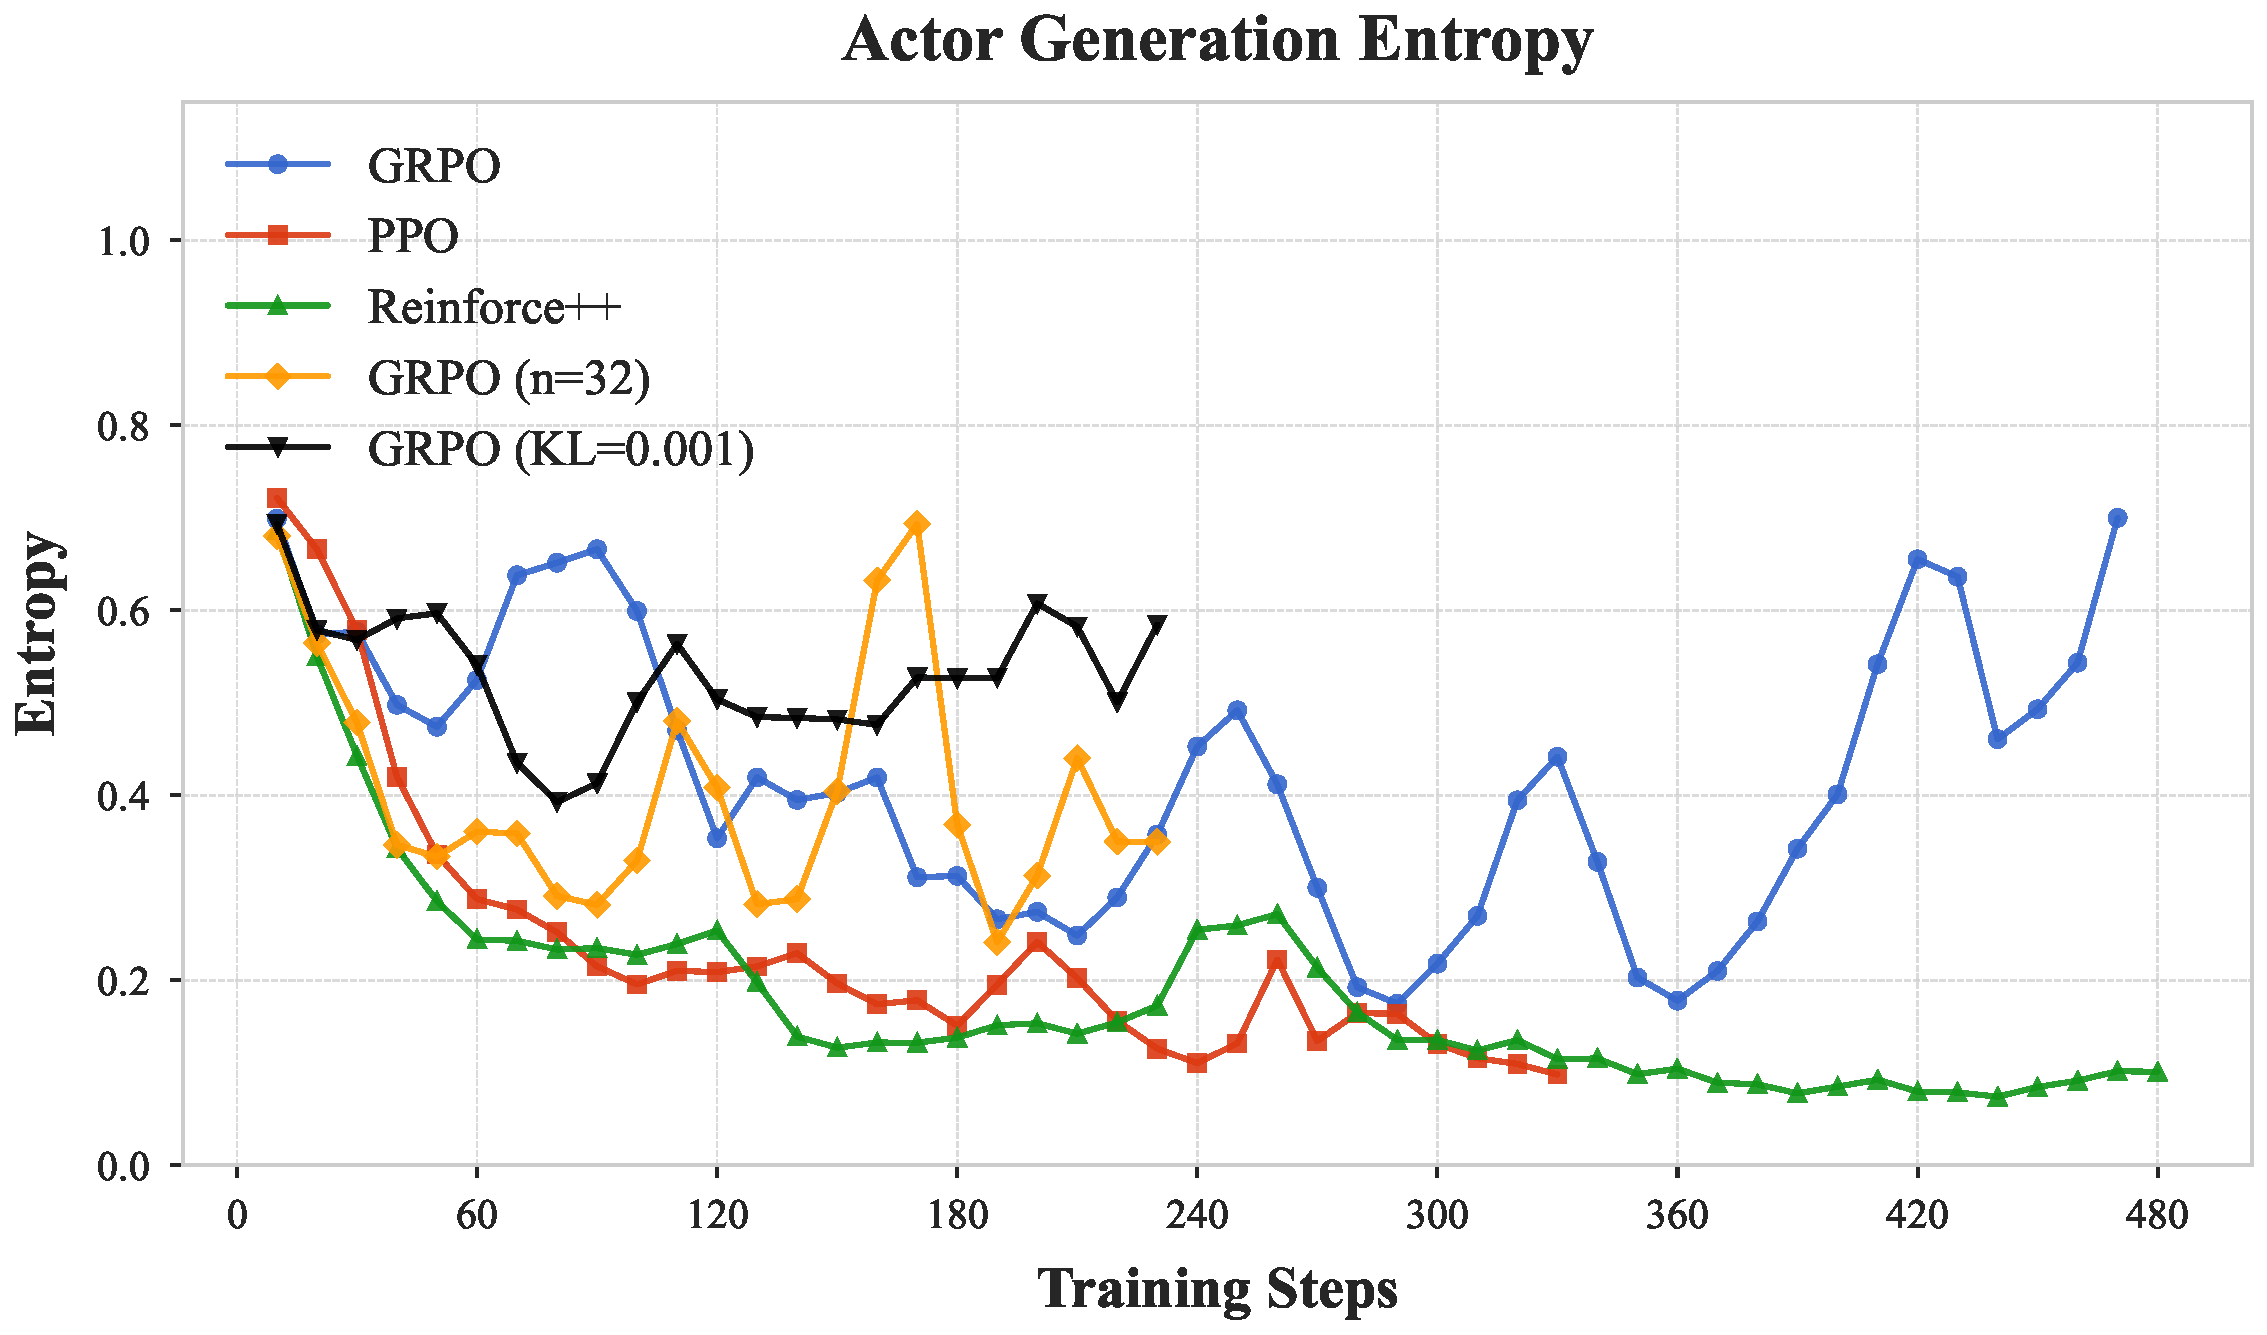
\includegraphics[width=\textwidth]{tex/images/dynamics_actor_entropy.pdf}
  \end{subfigure}
\caption{
The curves of training reward, response length, and generation entropy during training, corresponding to experiments in~\cref{sec:deep_analysis}. 
}
\label{fig:training_curves}
\vspace{-3mm}
\end{figure}


\clearpage
\subsection{CoT Case Analysis}

\begin{figure}[H]
  \centering
  \begin{subfigure}[b]{0.8\textwidth}
    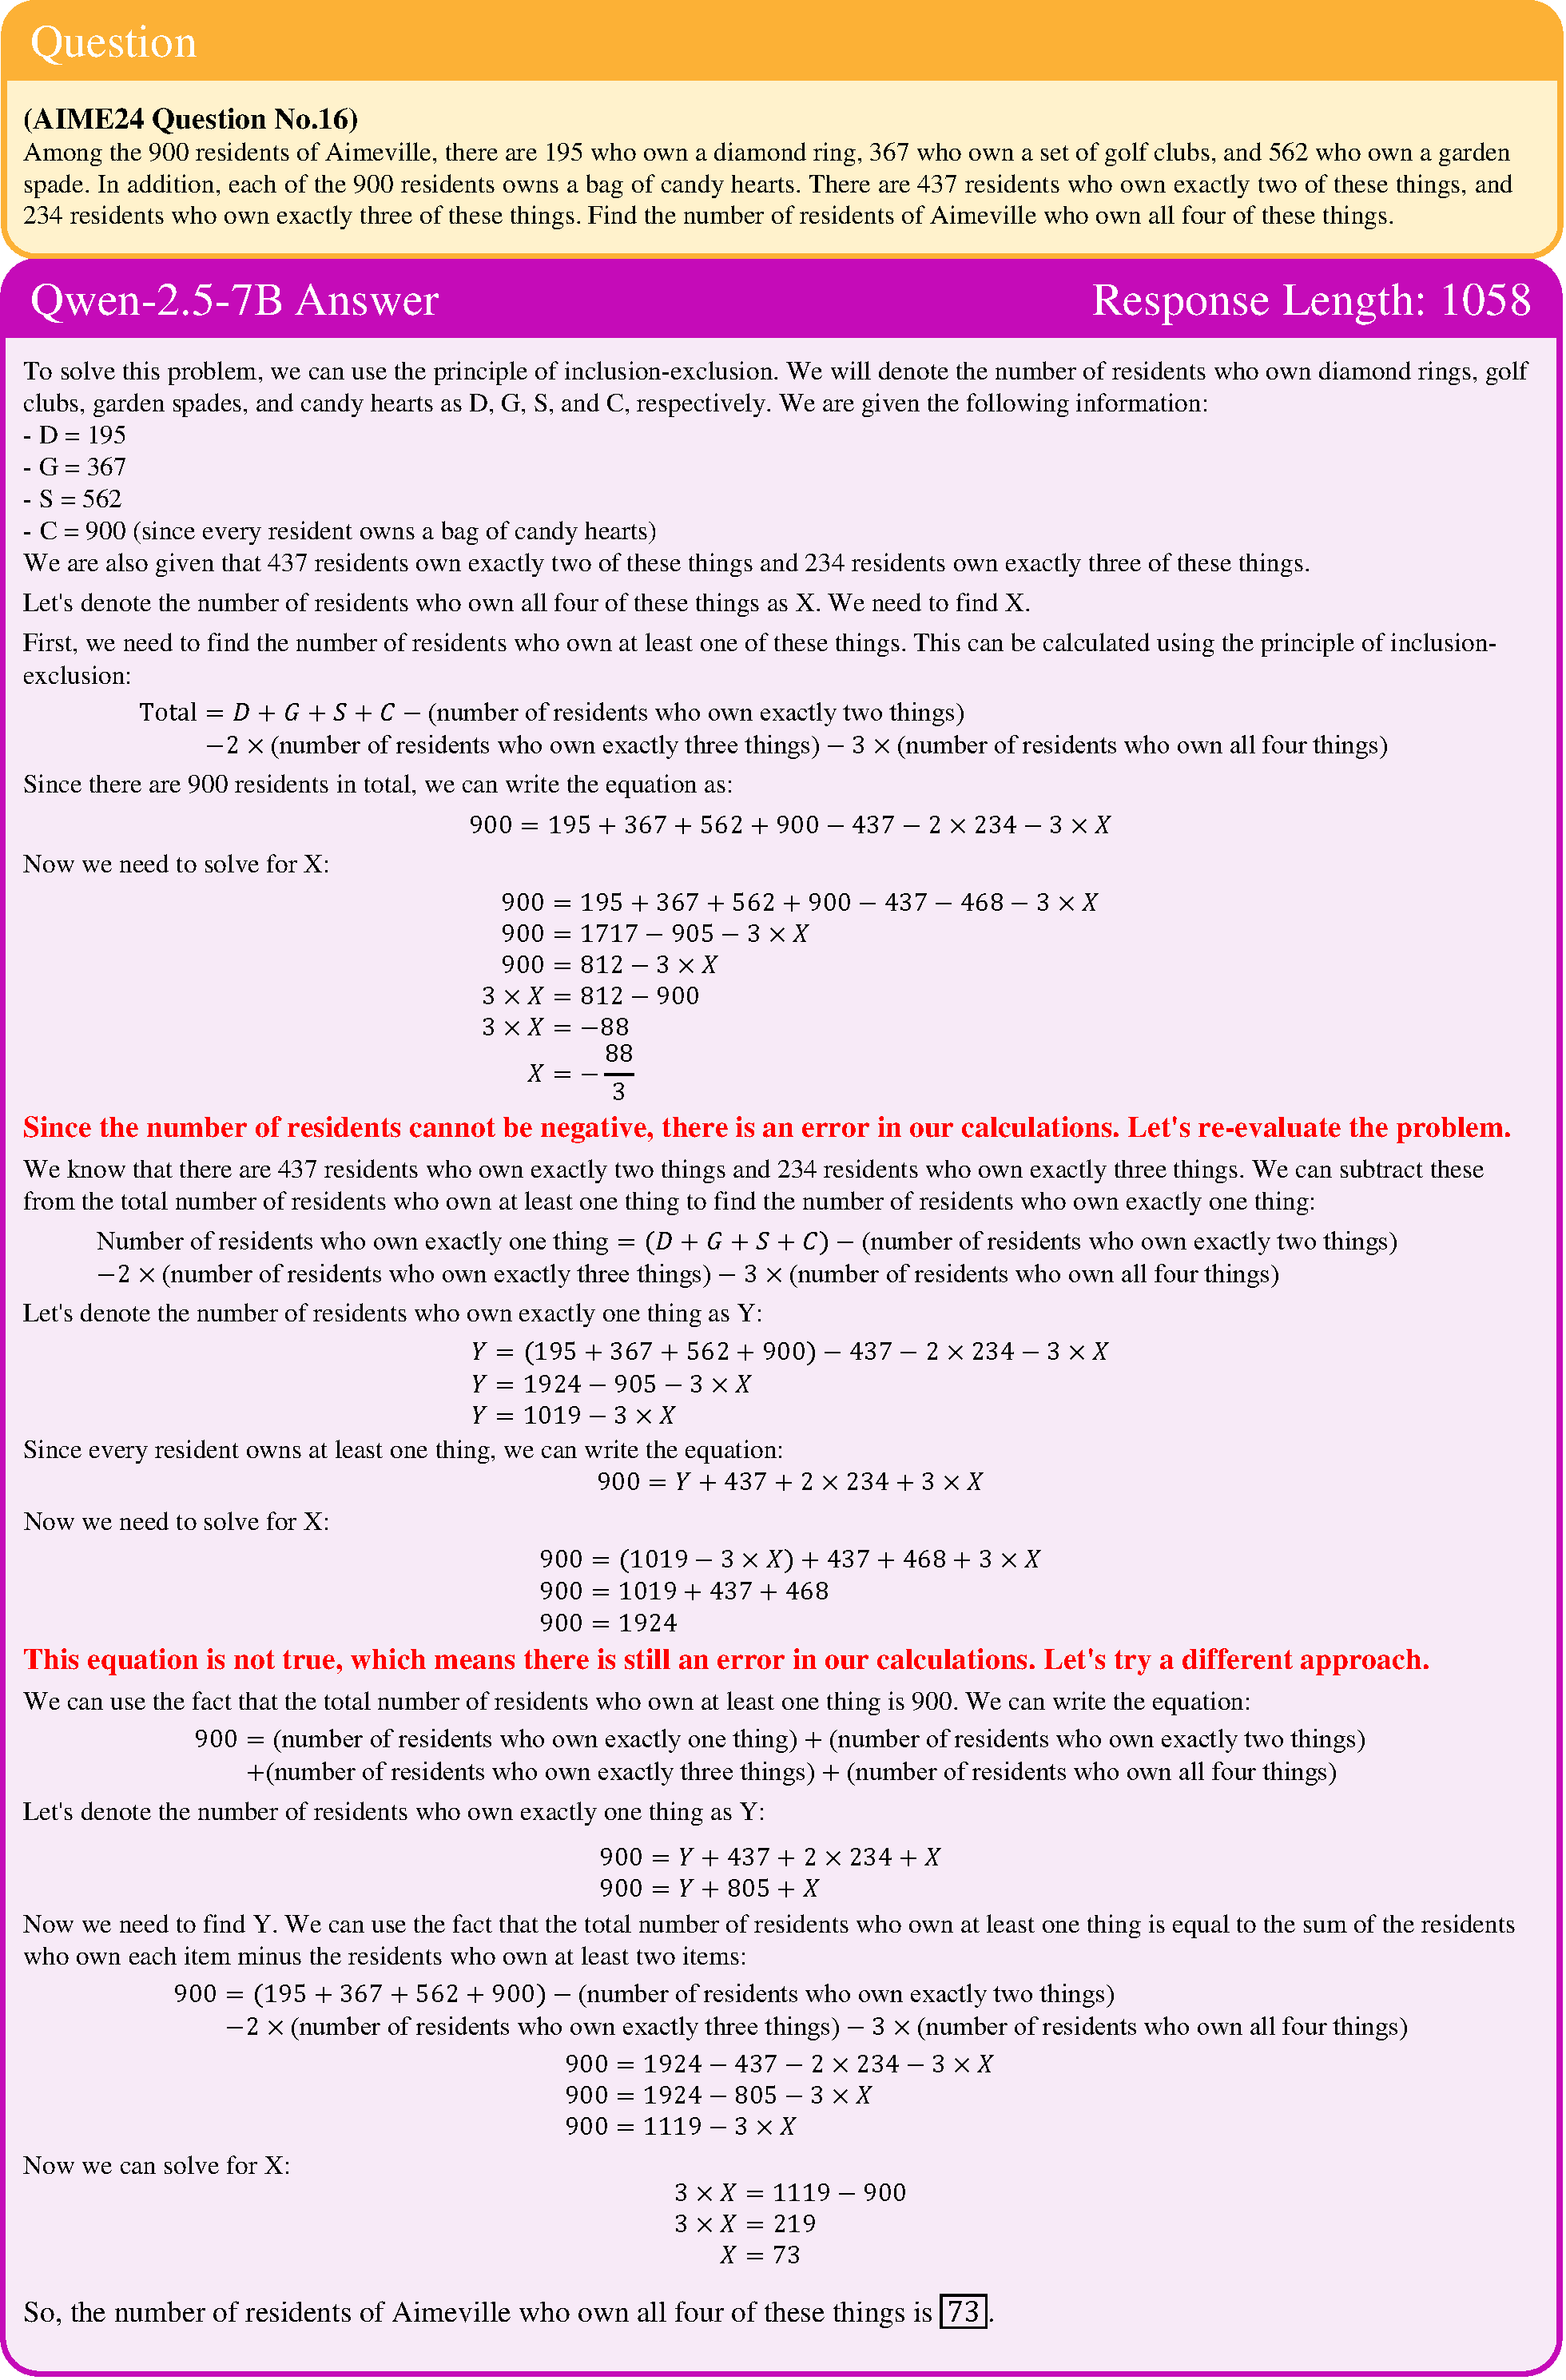
\includegraphics[width=\textwidth]{tex/images/AIME24_16_Base_Answer.pdf}
  \end{subfigure}
% \captionsetup{font={footnotesize}}
\caption{Qwen2.5-Base-7B Correct Response - Case 1.}
\label{fig:AIME24_16_Base_Answer}
\vspace{-3mm}
\end{figure}

\begin{figure}[h]
  \centering
  \begin{subfigure}[b]{0.85\textwidth}
    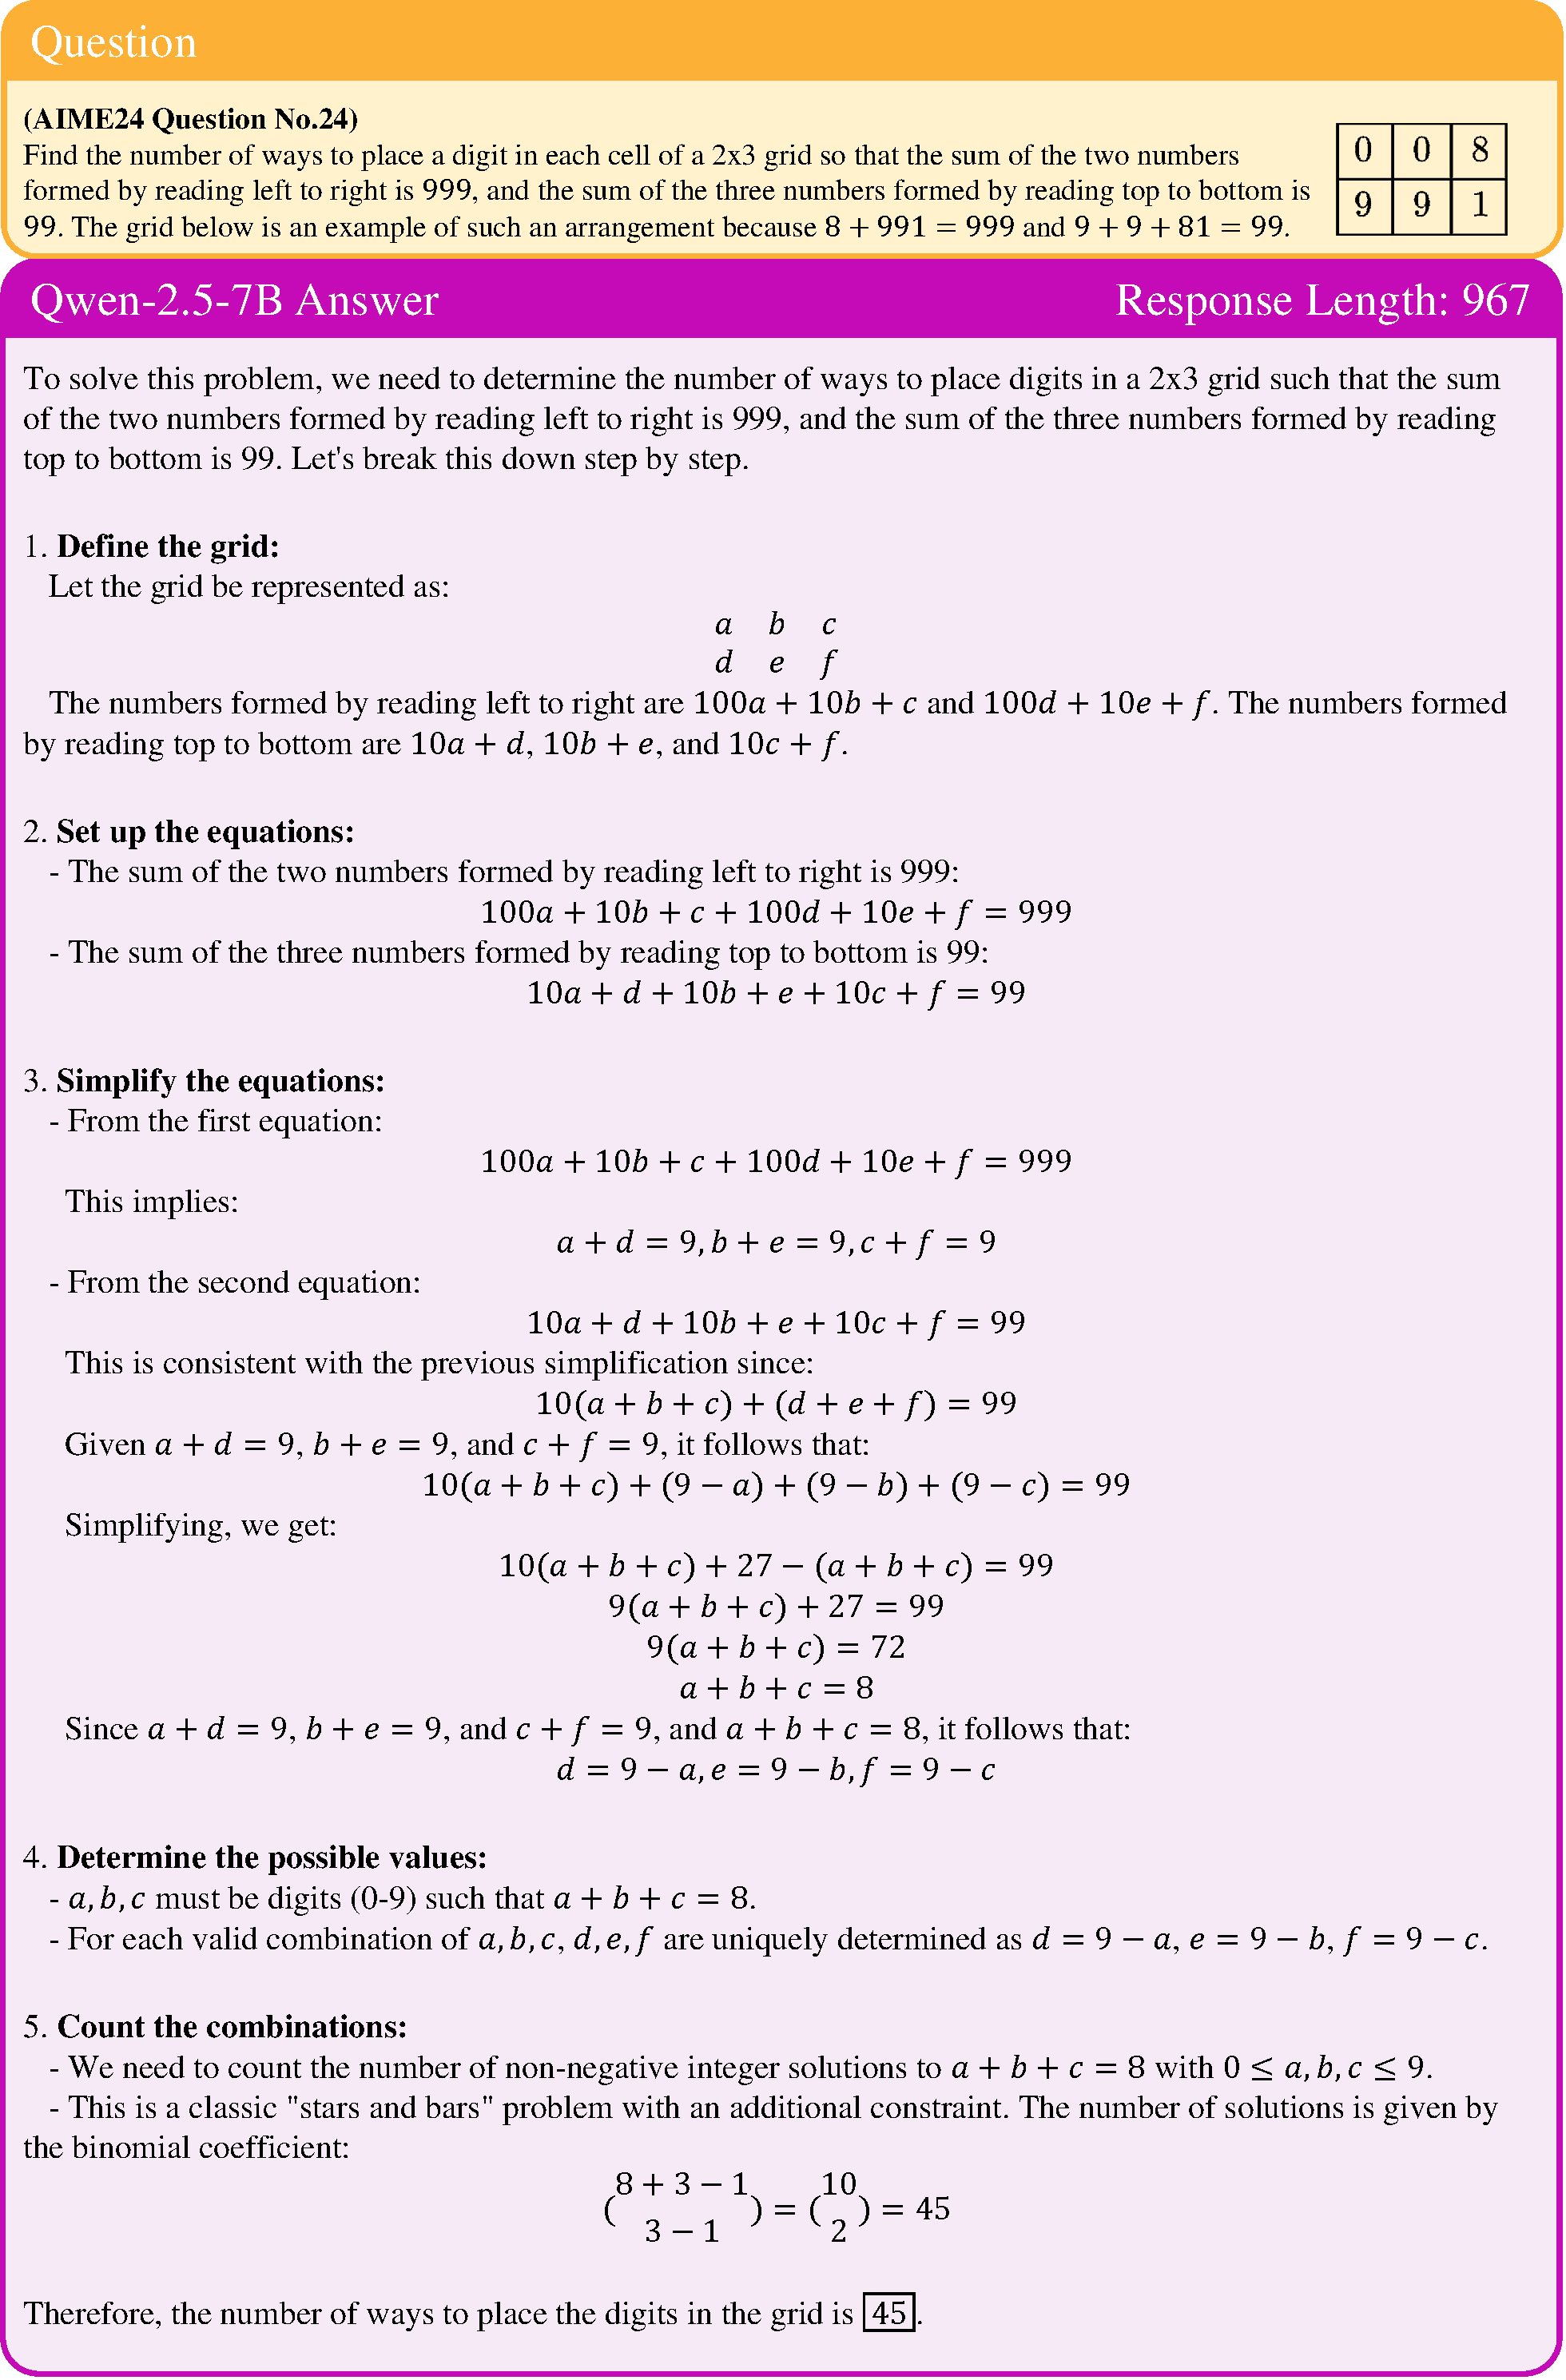
\includegraphics[width=\textwidth]{tex/images/AIME24_24_Base_Answer.pdf}
  \end{subfigure}
% \captionsetup{font={footnotesize}}
\caption{Qwen2.5-Base-7B Correct Response - Case 2.}
\label{fig:AIME24_24_Base_Answer}
\vspace{-3mm}
\end{figure}


\clearpage
\section{Prompt Templates}
\label{appendix:prompt}
We provide the prompt templates used for training and evaluation in our experiments. 
The prompt for SimpleRL training and evaluation is shown in~\cref{fig:SimpleRL_prompt}, while the prompt for Oat-Zero is shown in~\cref{fig:Oat_prompt}. 
For Code-R1 training, prompt in~\cref{fig:Code-R1_prompt} is adopted.
For Code-R1 evaluation, we follow the original codebase and adopt the default templates from the benchmarks, including LiveCodeBench prompt (\cref{fig:LiveCodeBench_prompt}), HumanEval+, and MBPP+ prompt (\cref{fig:humaneval+_Prompt}). 
The prompt used for EasyR1 training and evaluation is shown in~\cref{fig:EasyR1_prompt}. 
For VeRL-trained RL models, as discussed in~\cref{sec:algos} and~\cref{sec:steps}, the training and evaluation prompts are provided in~\cref{fig:VeRL_Training_and Evaluation_Prompt}. 
For evaluating Mistral and Magistral models on AIME24/25, prompts are provided in~\cref{fig:mistral_Prompt}.
To ensure a fair comparison, the base models use the same prompts as their corresponding RL-trained counterparts during evaluation.


\begin{figure}[h]
  \vspace{4mm}
  \centering
  \begin{subfigure}[b]{0.7\textwidth}
    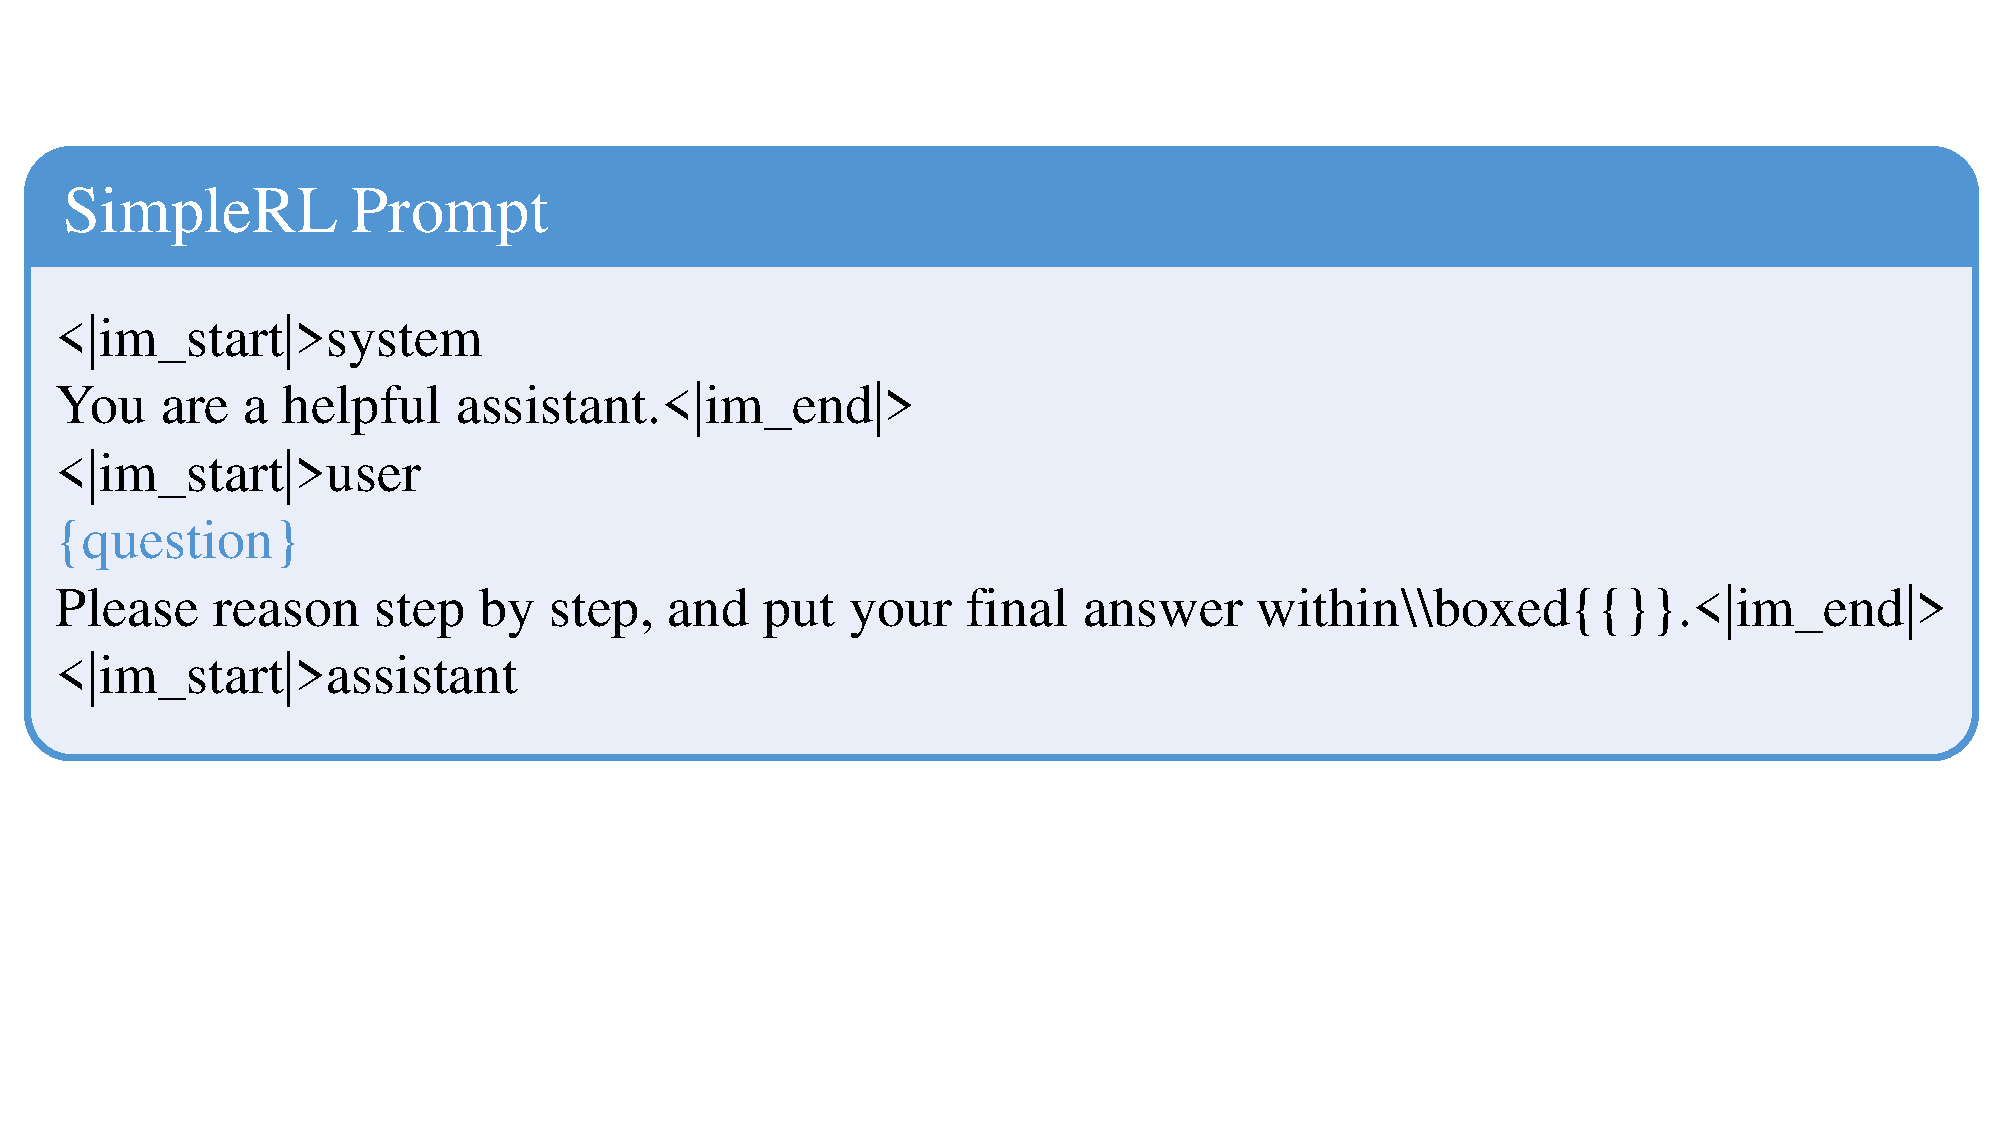
\includegraphics[width=\textwidth]{tex/images/SimpleRL_prompt.pdf}
  \end{subfigure}
% \captionsetup{font={footnotesize}}
\caption{
Prompt for SimpleRL Training and Evaluation.
The base model uses the same prompt as the RL model during evaluation.
}
\label{fig:SimpleRL_prompt}
% \vspace{-3mm}
\end{figure}


% oat

\begin{figure}[h]
  \centering
  \begin{subfigure}[b]{0.7\textwidth}
    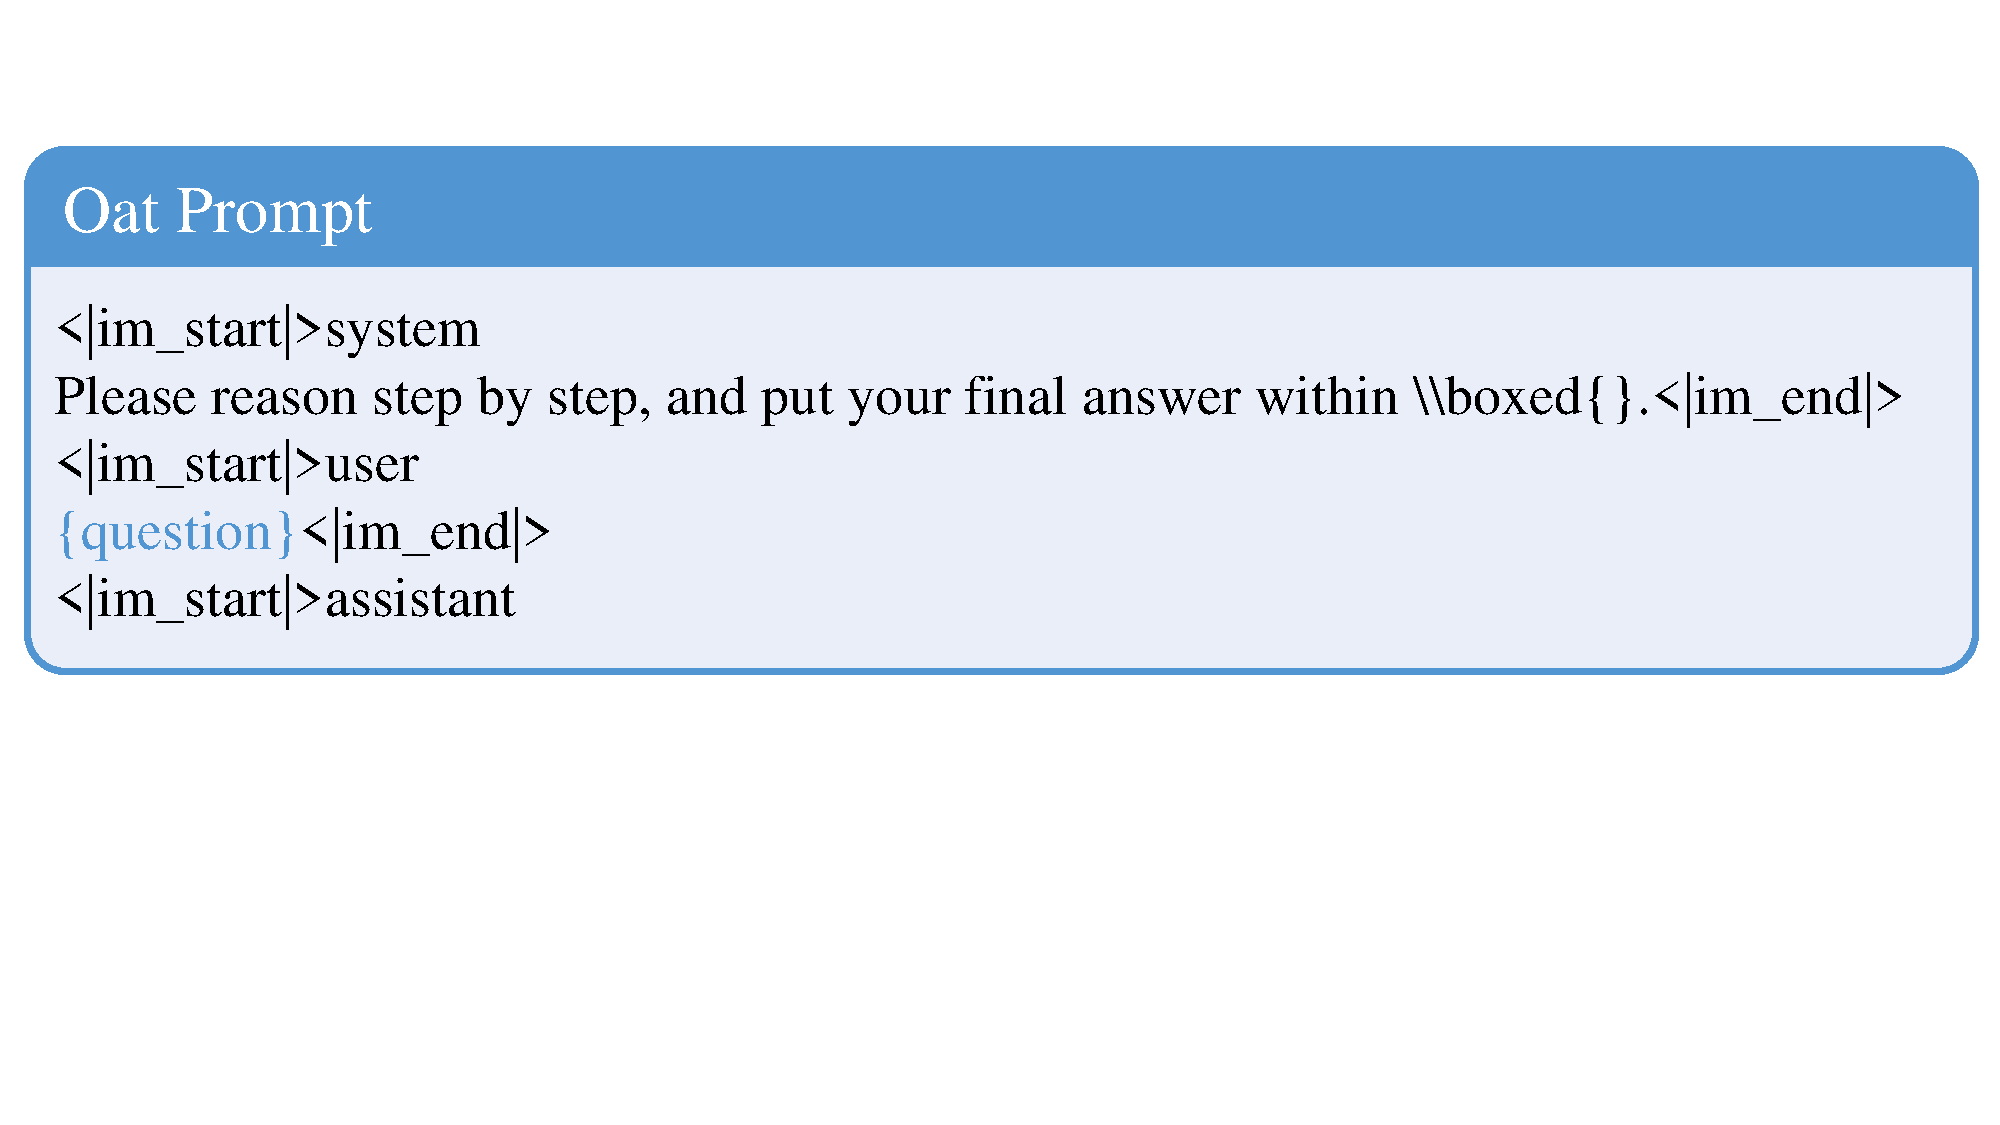
\includegraphics[width=\textwidth]{tex/images/Oat_prompt.pdf}
  \end{subfigure}
% \captionsetup{font={footnotesize}}
\vspace{-1mm}
\caption{
Prompt for Oat-Zero training and evaluation.
}
\label{fig:Oat_prompt}
% \vspace{-3mm}
\end{figure}


\begin{figure}[h]
  \centering
  \begin{subfigure}[b]{0.7\textwidth}
    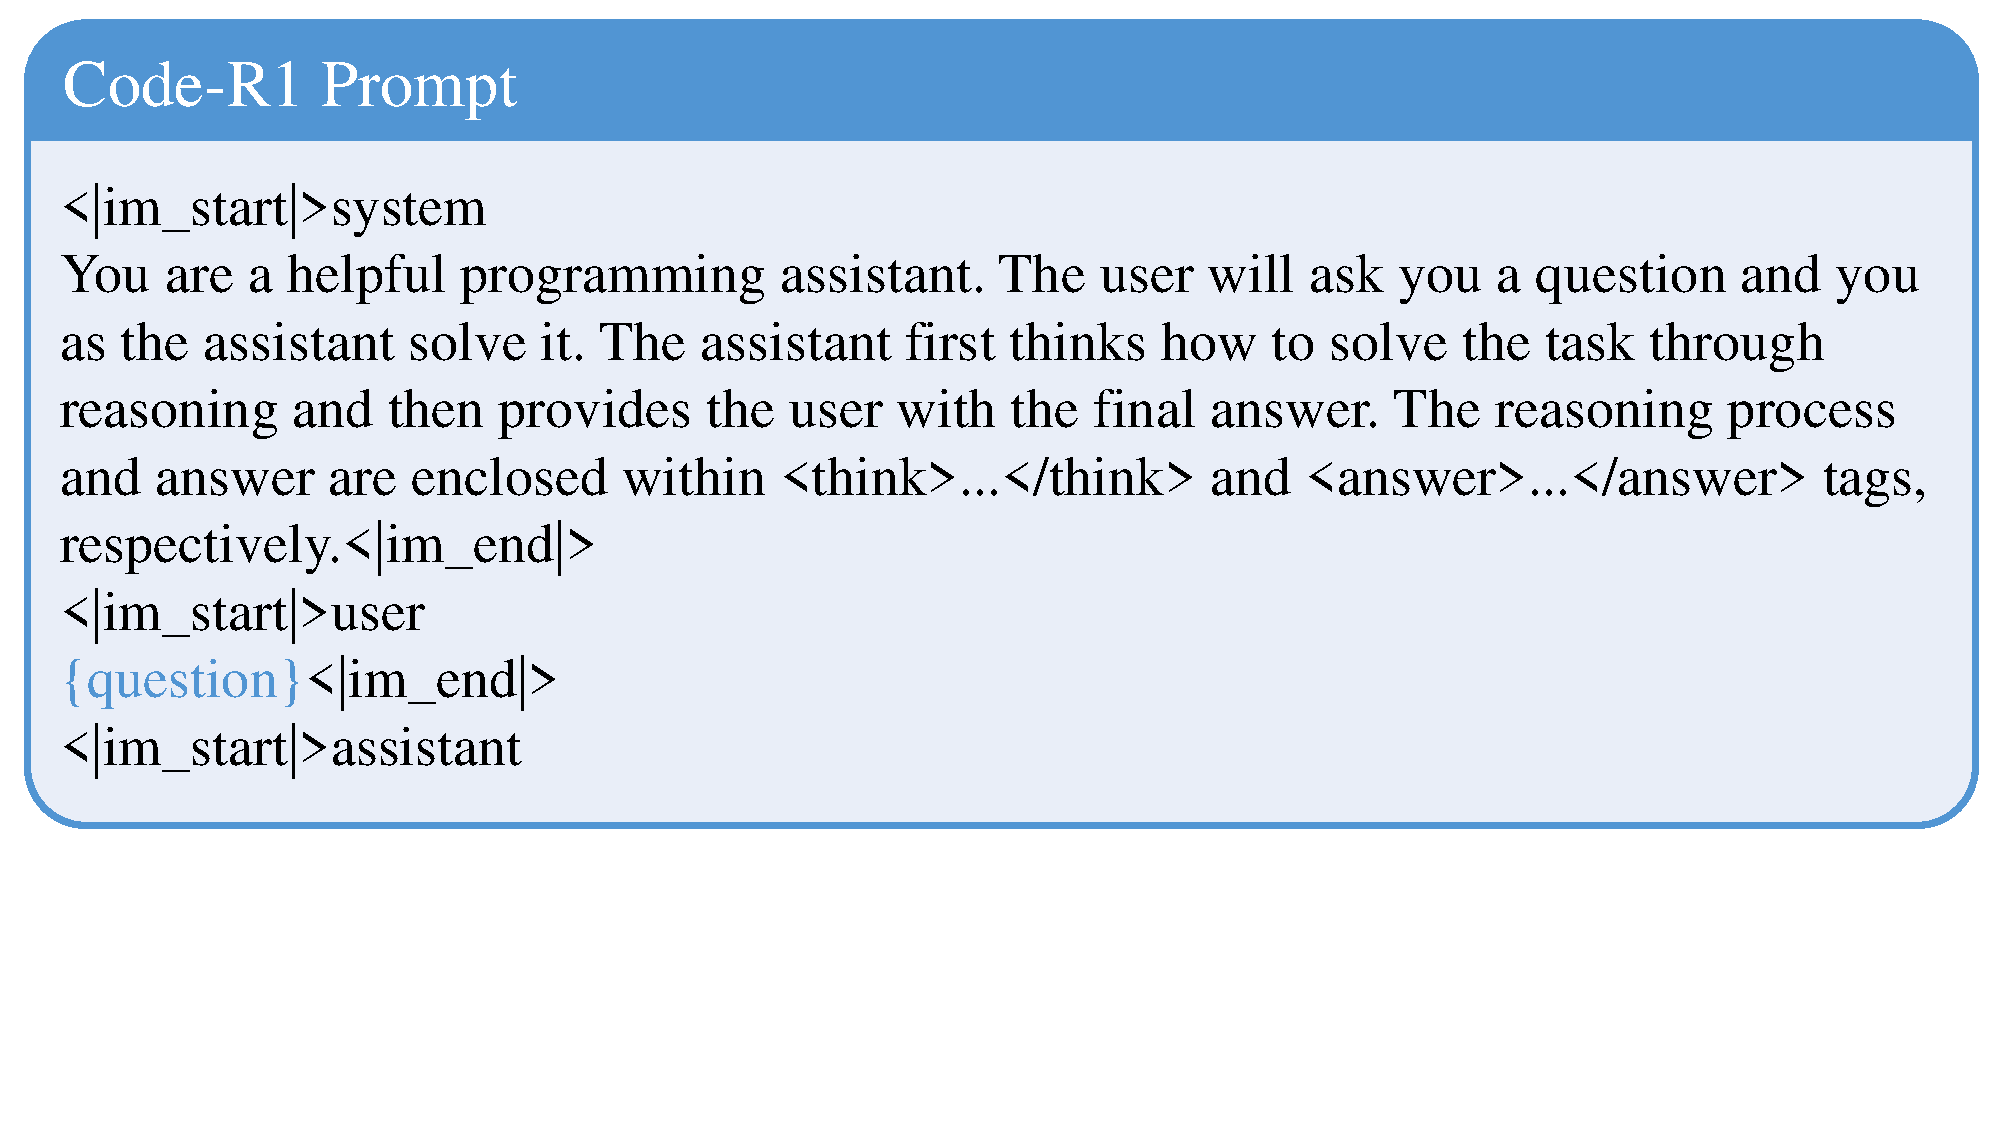
\includegraphics[width=\textwidth]{tex/images/Code-R1_prompt.pdf}
  \end{subfigure}
% \captionsetup{font={footnotesize}}
\vspace{-1mm}
\caption{
Prompt for Code-R1 training.
}
\label{fig:Code-R1_prompt}
% \vspace{-3mm}
\end{figure}


\begin{figure}[h]
  \centering
  \begin{subfigure}[b]{0.7\textwidth}
    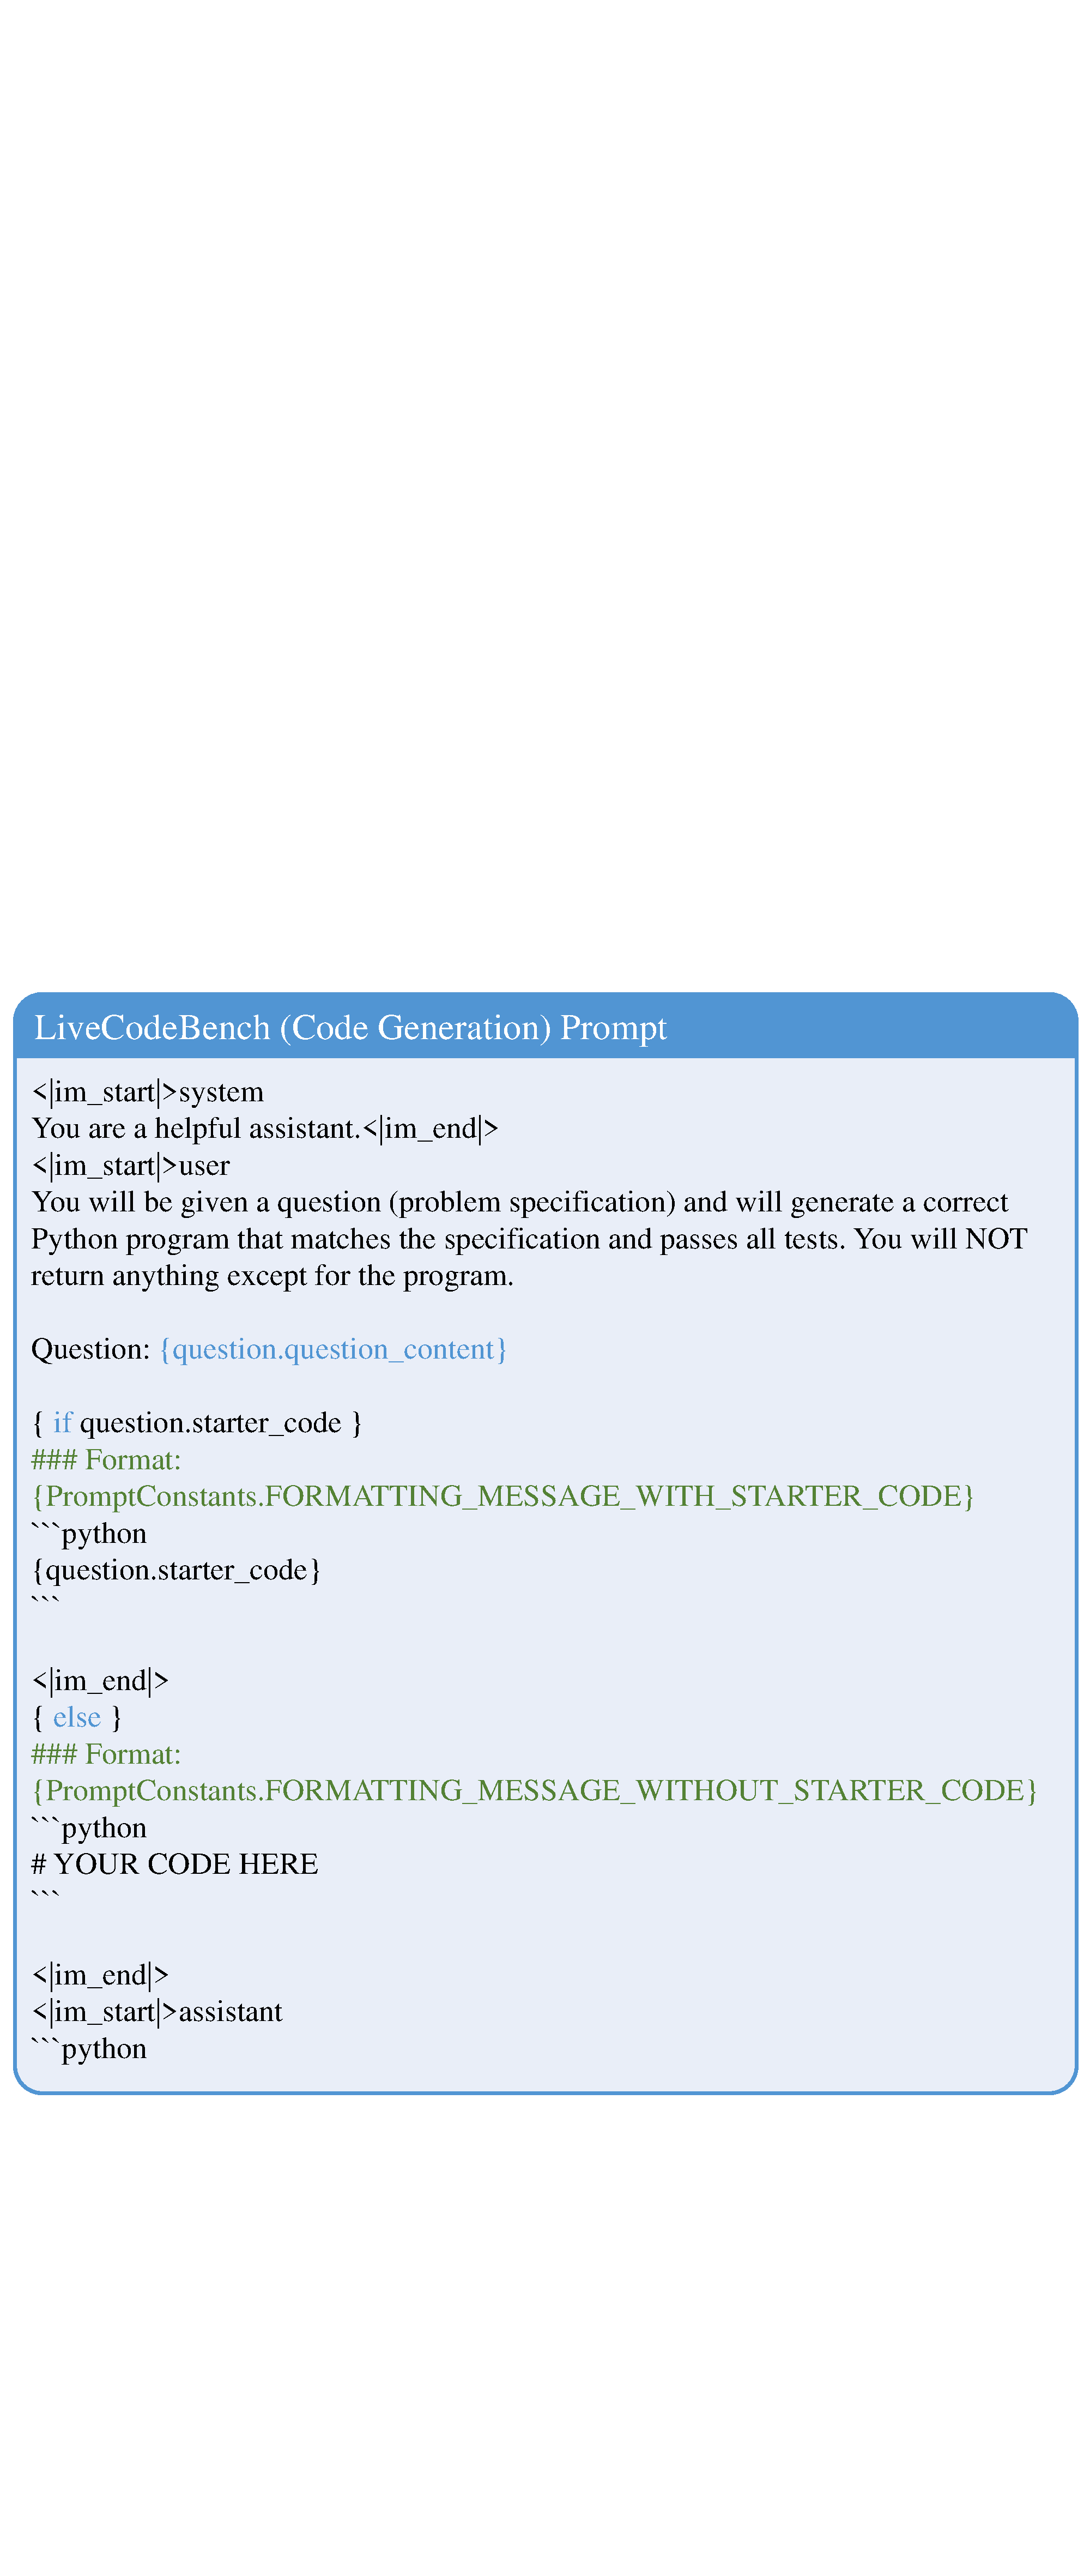
\includegraphics[width=\textwidth]{tex/images/LiveCodeBench_prompt.pdf}
  \end{subfigure}
% \captionsetup{font={footnotesize}}
\vspace{-1mm}
\caption{
Since Code-R1 does not specify an evaluation prompt, we adopt the original LiveCodeBench evaluation prompt. To encourage both the base and RL-trained models to generate code, we append \texttt{```python} to the end of the prompt. Using this setup, we reproduce a pass@$1$ score of 28.6, which is close to the reported 29.7.
}
\label{fig:LiveCodeBench_prompt}
% \vspace{-3mm}
\end{figure}

\begin{figure}[h]
  \centering
  \begin{subfigure}[b]{0.7\textwidth}
    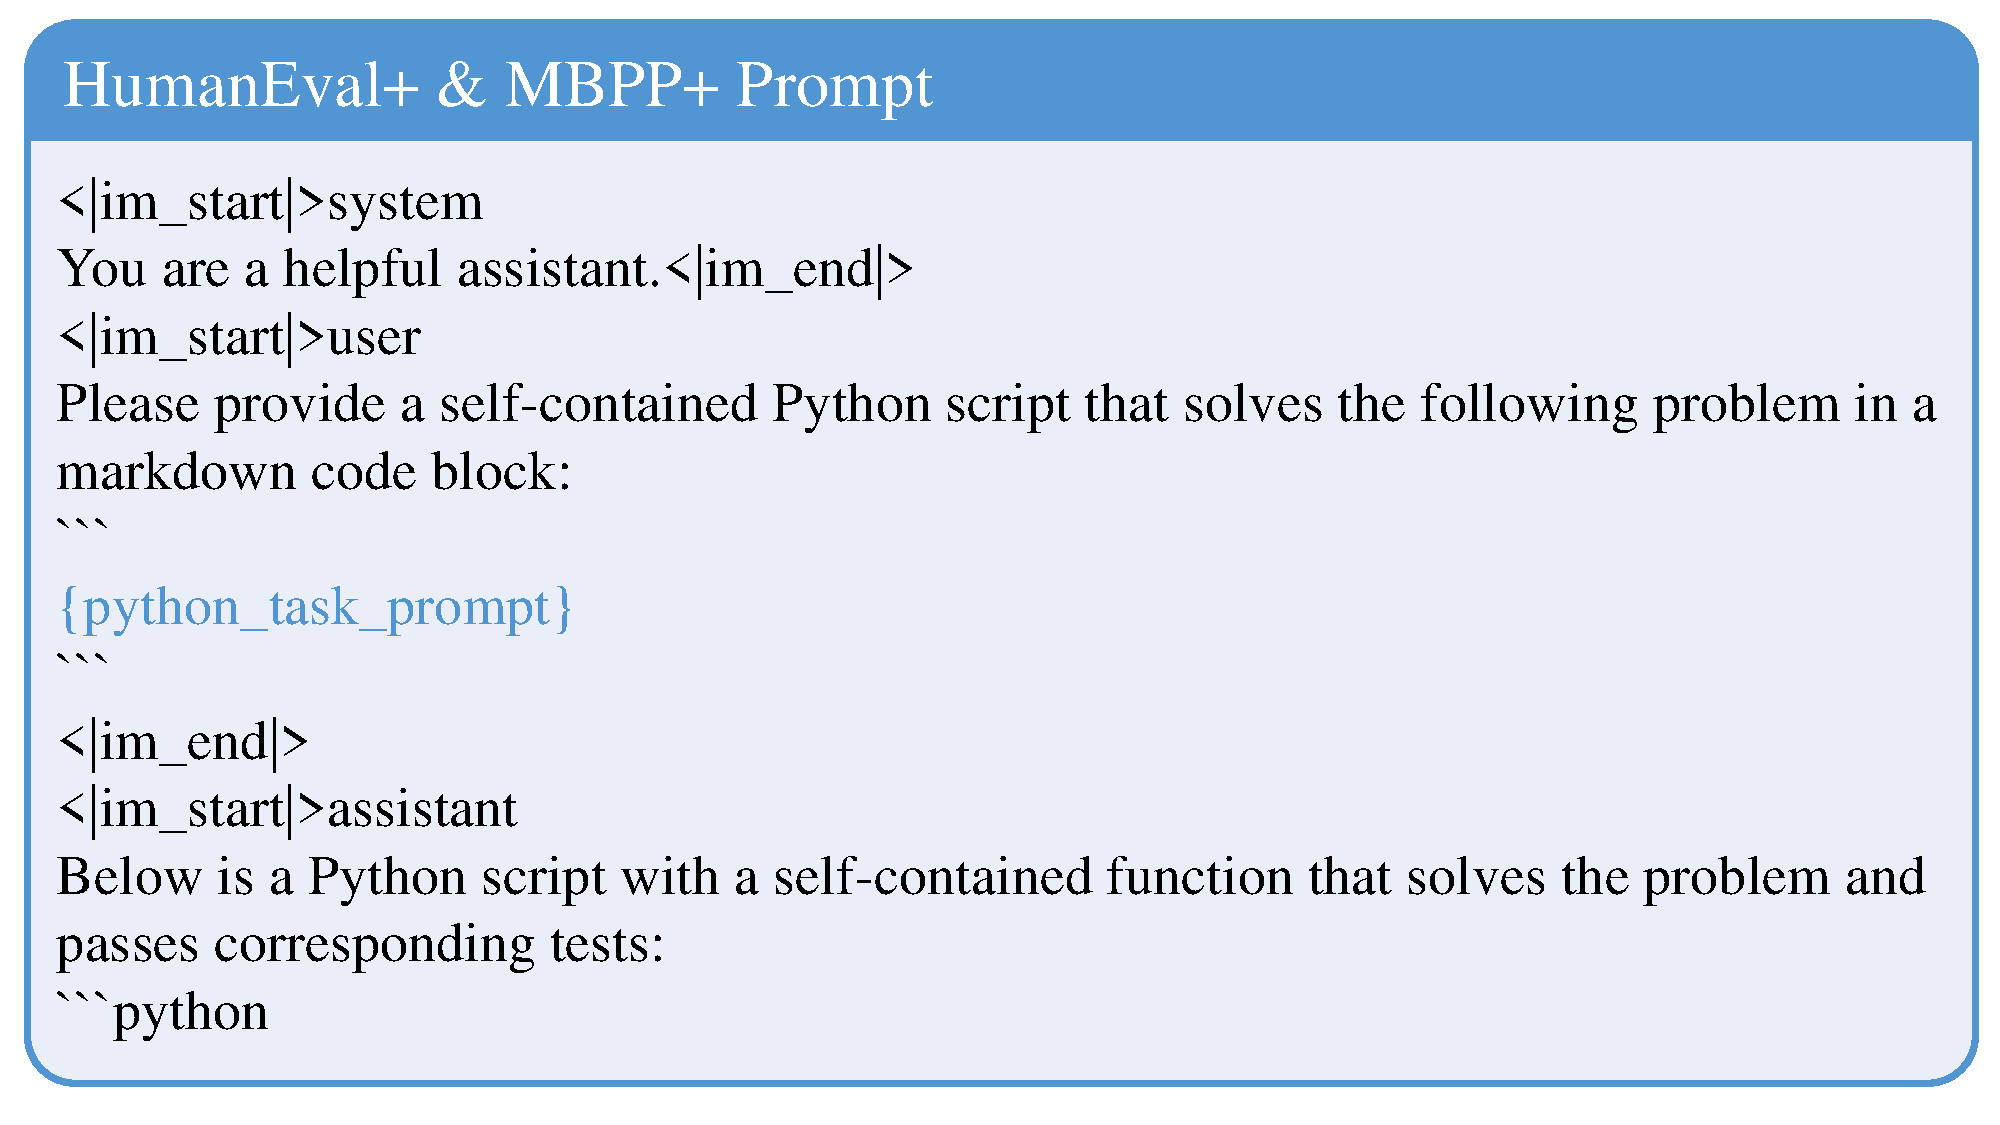
\includegraphics[width=\textwidth]{tex/images/HumanEval+_prompt.pdf}
  \end{subfigure}
% \captionsetup{font={footnotesize}}
\caption{
Prompt for Code-R1 Evaluation on HumanEval+ and MBPP+.
}
\label{fig:humaneval+_Prompt}
\vspace{-3mm}
\end{figure}

\clearpage

\begin{figure}[!h]
  \centering
  \begin{subfigure}[b]{0.7\textwidth}
    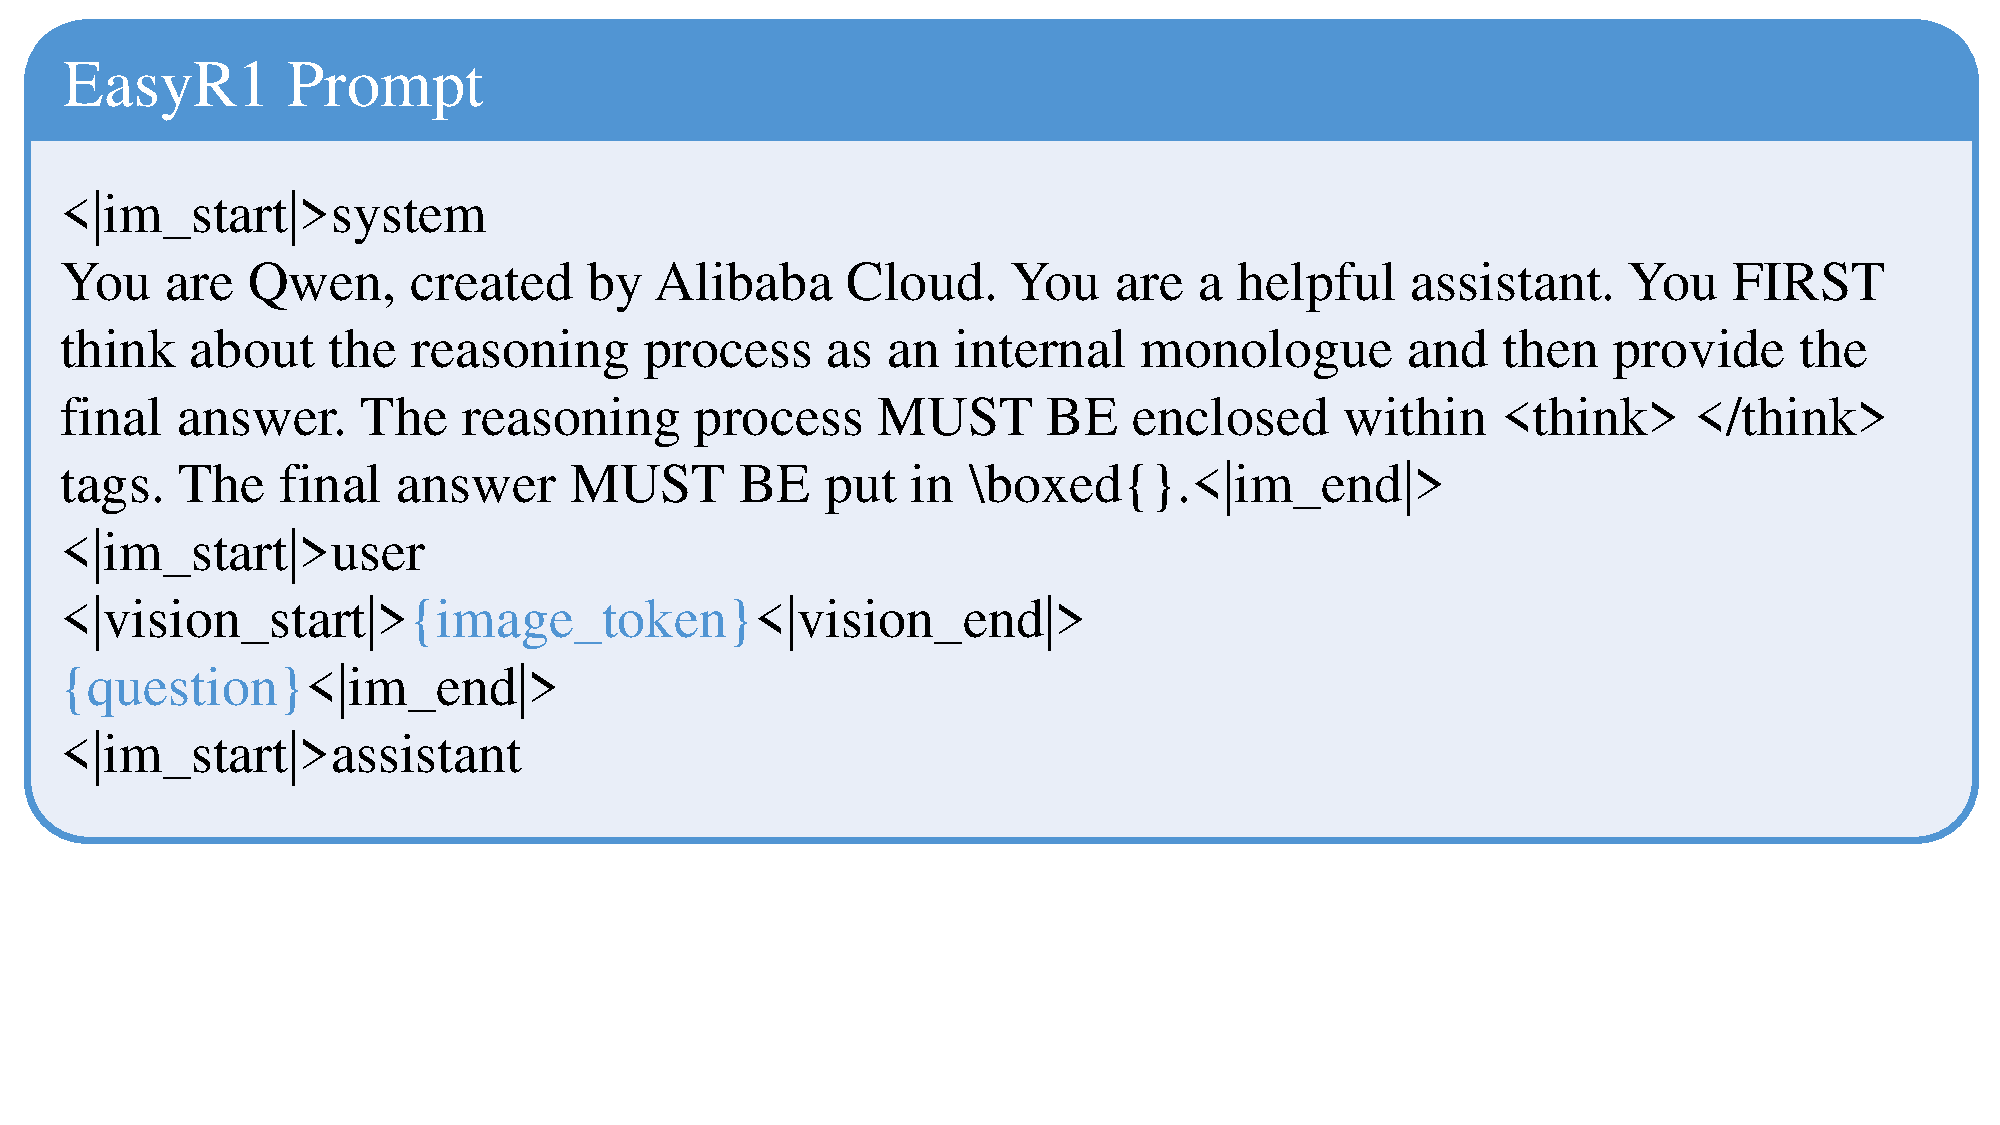
\includegraphics[width=\textwidth]{tex/images/EasyR1_prompt.pdf}
  \end{subfigure}
% \captionsetup{font={footnotesize}}
\caption{
Prompt for EasyR1 training and evaluation.
}
\label{fig:EasyR1_prompt}
\vspace{-3mm}
\end{figure}

\begin{figure}[!h]
  \centering
  \begin{subfigure}[b]{0.7\textwidth}
    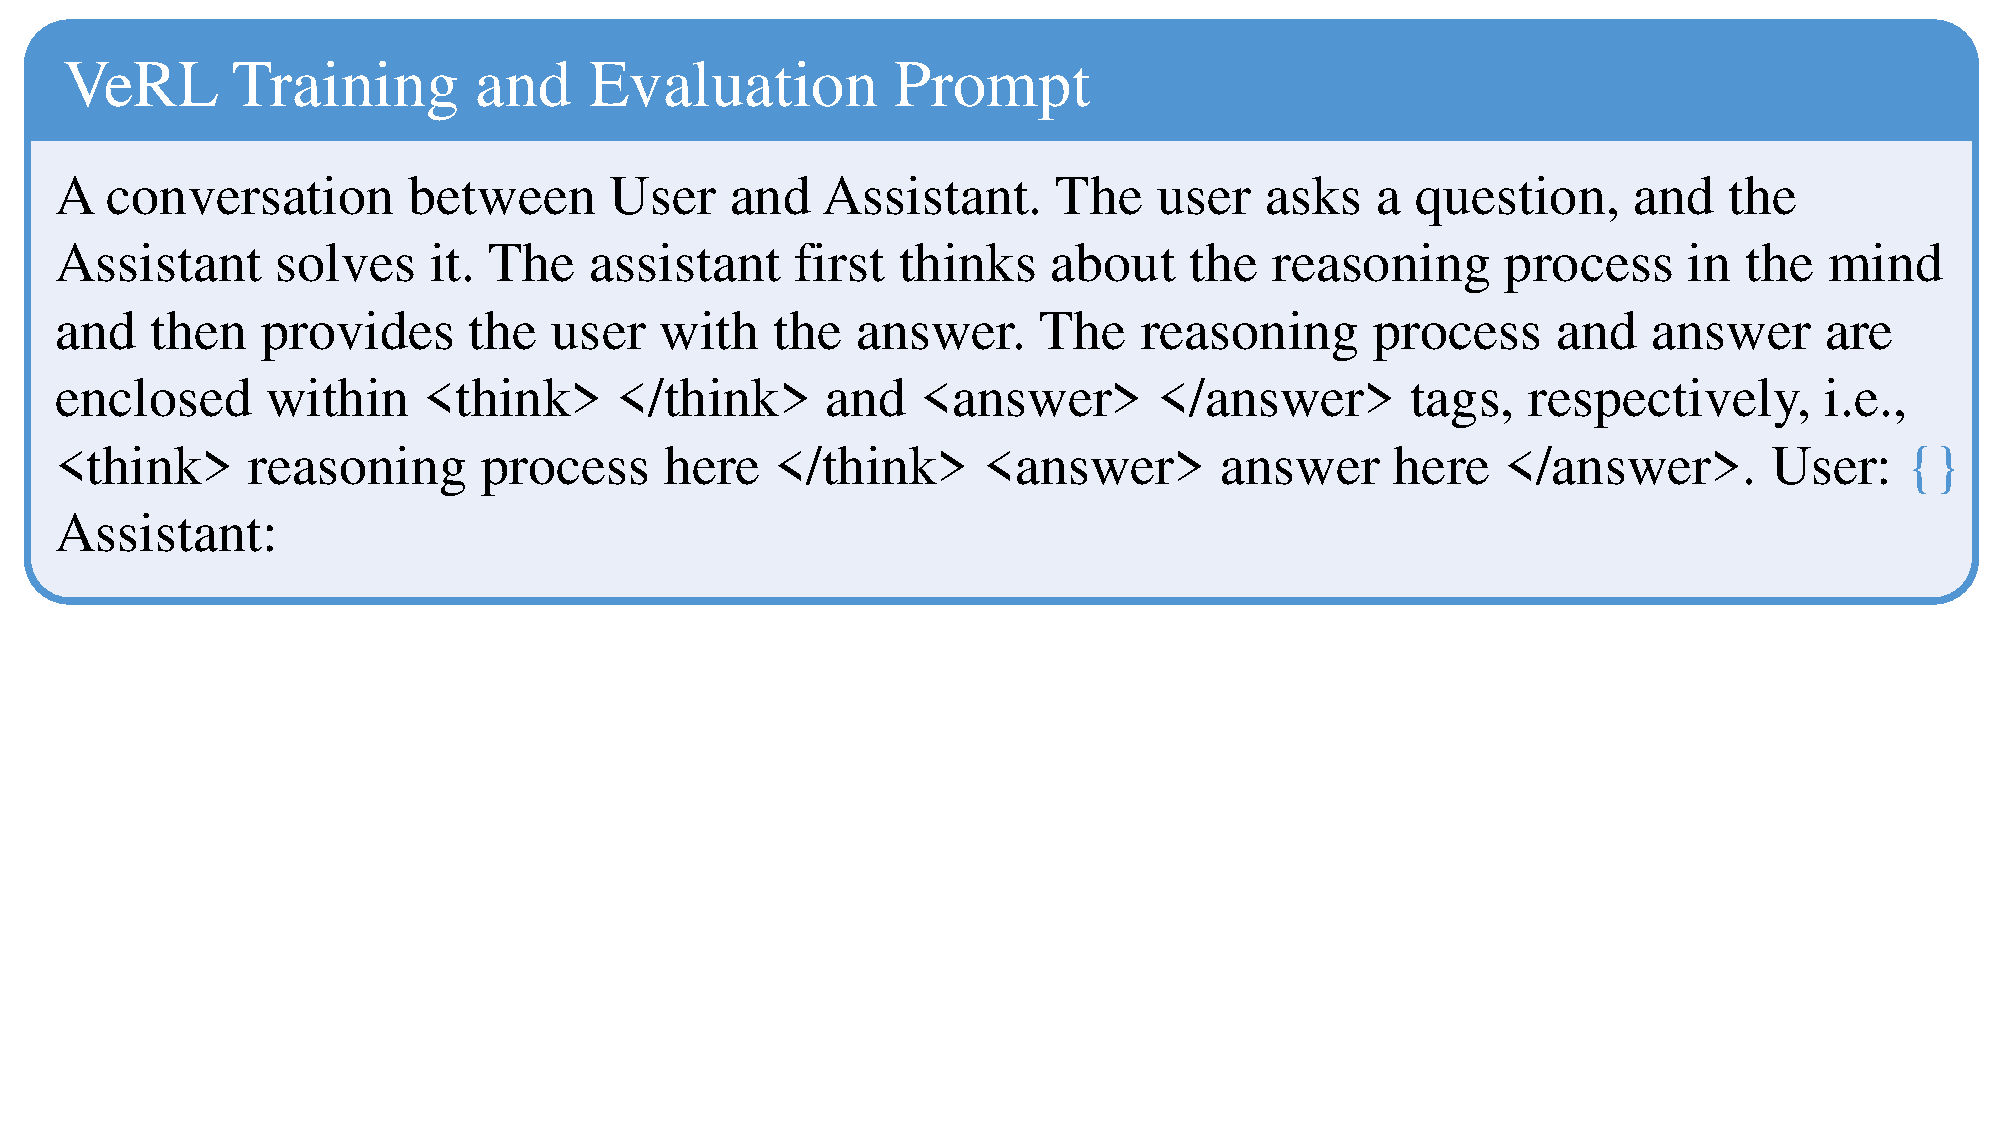
\includegraphics[width=\textwidth]{tex/images/VeRL_Training_and_Evaluation_Prompt.pdf}
  \end{subfigure}
% \captionsetup{font={footnotesize}}
\caption{
Prompt for VeRL training on Omni-math-train and evaluation on Omni-math-eval and MATH500.
}
\label{fig:VeRL_Training_and Evaluation_Prompt}
\vspace{-3mm}
\end{figure}


\begin{figure}[!h]
  \centering
  \begin{subfigure}[b]{0.7\textwidth}
    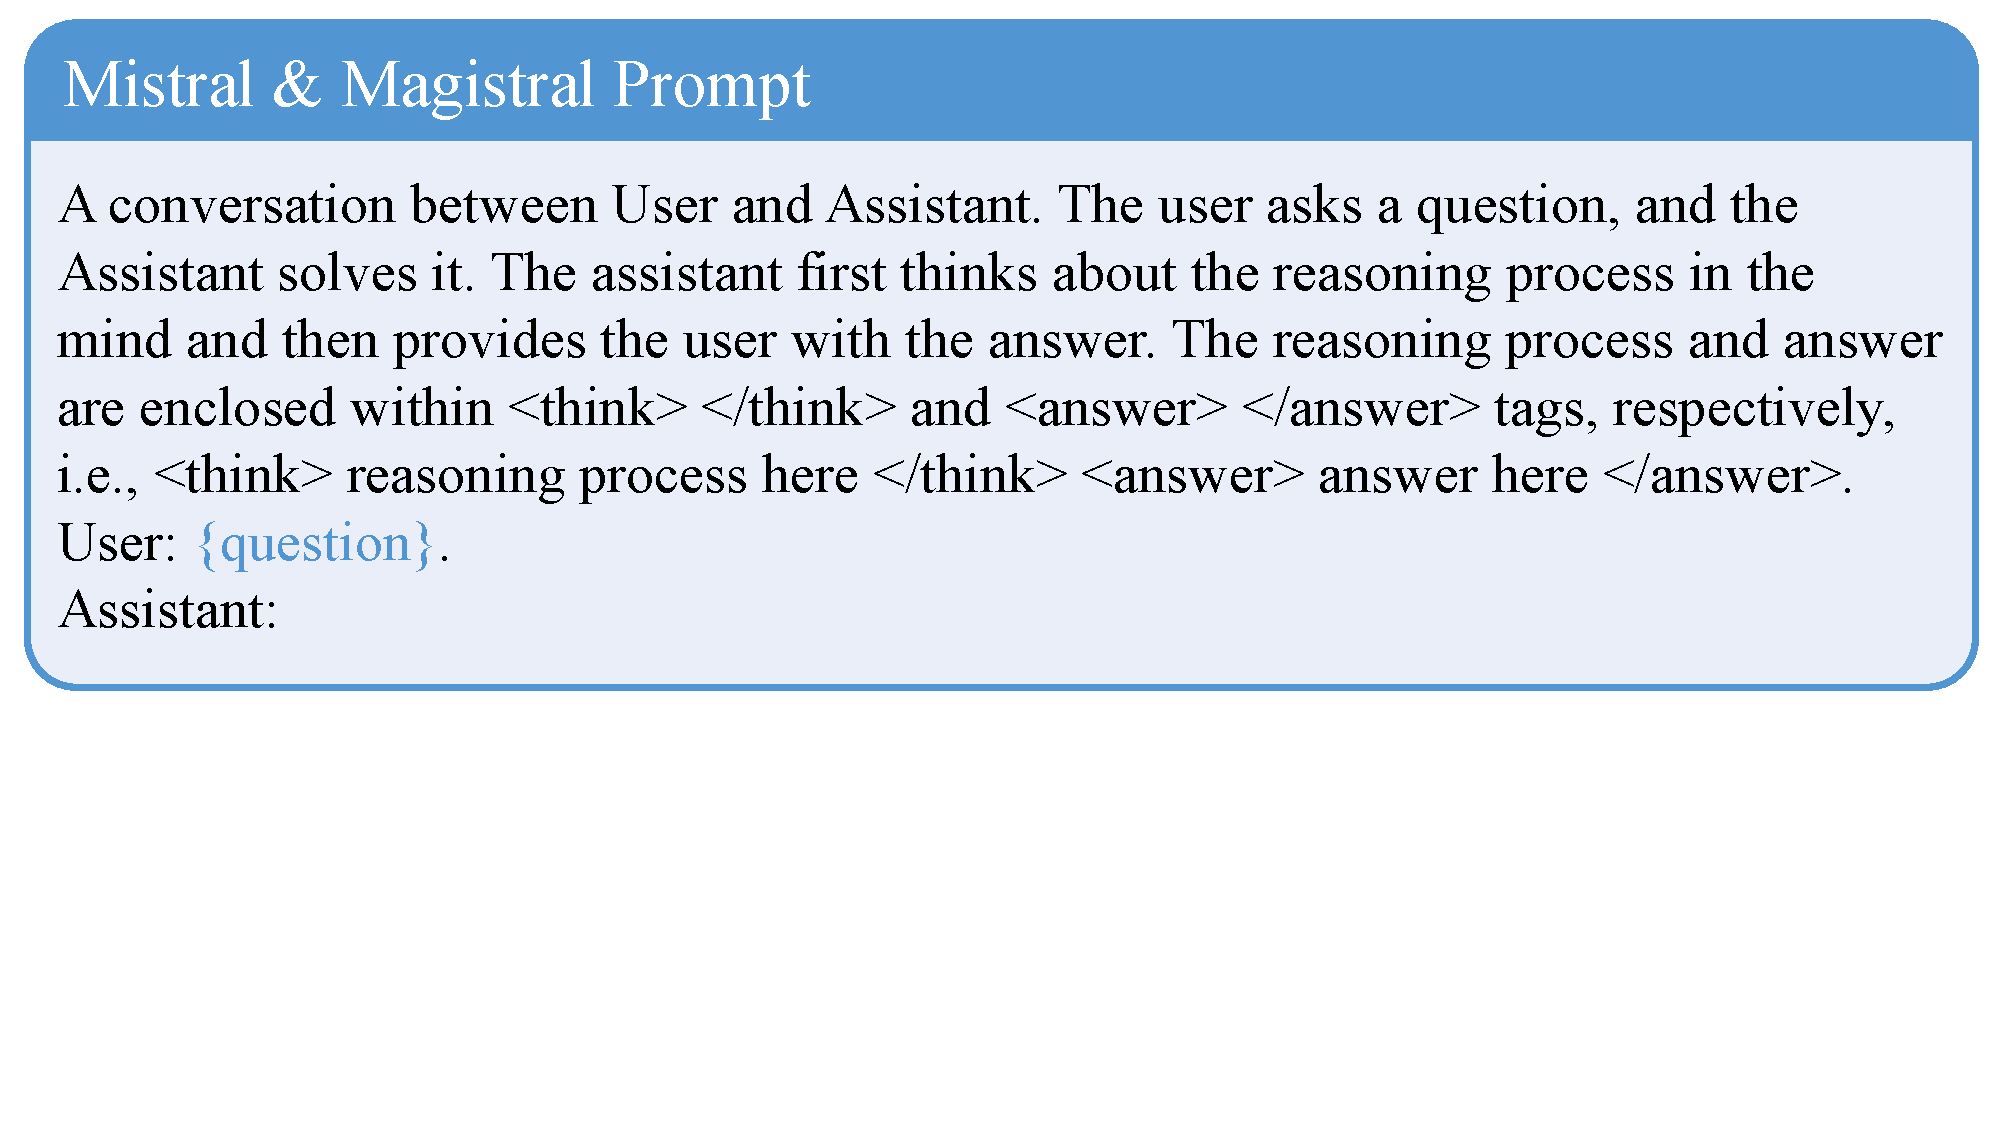
\includegraphics[width=\textwidth]{tex/images/Mistral_prompt.pdf}
  \end{subfigure}
% \captionsetup{font={footnotesize}}
\caption{
Prompt for Mistral and Magistral model evaluation.
}
\label{fig:mistral_Prompt}
\vspace{-3mm}
\end{figure}

\section{Broader Impacts}
The potential negative social impacts of our method align with those typically associated with general LLM reasoning technologies. We emphasize the importance of adhering to the principles of fair and safe deployment in LLM systems. 